%!TEX root = ../swiatlow_thesis.tex
\label{chapter:detector}

The design of the LHC, with two high-luminosity interaction points at opposite ends of the ring, called for two general purpose detectors to be built in these locations. Their charge was to accurately reconstruct collision events in the most hostile conditions yet seen in a collider: with a bunch spacing of 25 ns and the unprecedented introduction of pile-up, the detectors would have an enormous challenge ahead of them in dealing with both the rate and the reconstruction of events. ATLAS (A Toroidal LHC APparatus)~\cite{ATLASPaper} and CMS (Compact Muon Solenoid)~\cite{CMSPaper} were the two detectors built for this task, with ATLAS occupying the (much more convenient) Point 1 and CMS located at the (very distant) Point 5. The data presented in this thesis was collected by the ATLAS experiment in $pp$ collisions at $\sqrt{s} = 7$~TeV in 2011 and $\sqrt{s} = 8$~TeV in 2012.

The goal of a particle detector is to reconstruct collisions: outgoing particles are measured in some way, and 4-vectors corresponding to these particles are constructed. These 4-vectors are combined in various ways to understand the particles--- Higgs bosons, gluinos, and so on--- which were produced in the collision and subsequently decayed to the measured particles\footnote{At a hadron collider, this process is somewhat complicated by the misbalance in the $z$-direction of the incoming particles: as the $z$-momenta of the colliding quarks and gluons is not known (only that of the composite protons), it is often simplest to discuss the momenta only in the transverse plane (where the momenta of the incoming particles is known to be zero).}. But before this high level physics analysis can occur, the particles outgoing from the collision need to be measured.

Particle detectors measure particles via their interactions with matter, as drawn schematically in Figure~\ref{fig:detector:schematic}. For example, charged particles (such as electrons and some hadrons) interact electromagnetically with silicon and gas tubes, leaving hits in different layers of detectors which can be traced back to form a track. Electrons and photons, with their low masses and high rate of interaction with matter, are measured by the electromagnetic calorimeter. The calorimeter is composed of alternating layers of metal meant to cause the particle to interact and lose energy, and active materials which measure the energy left behind in these interactions. The hadron calorimeter follows a similar principle, and alternately placed layers of metal and active material again aim to stop and measure the hadrons which the electromagnetic calorimeter did not stop. Muons, which do not interact very much with matter most matter but do leave hits in trackers, survive past even the hadronic calorimeter, and a special set of muon detectors can be used to identify them there. Neutrinos, as they interact with matter only via the weak force and thus very rarely, escape detection and are reconstructed only by inferring their presence from the lack of momentum conservation in the transverse plane.

A significant constraint in the design of detectors is the interaction of particles with matter. As particles traverse matter--- including the detectors built to measure them--- they lose energy via interactions, or in the case of photons, can even convert into electron/positron pairs. As some detectors--- particularly the calorimeters--- sit radially behind others, this can mean that substantial portions of the energy of particles can have already dispersed by the time they are measured. One of the keys to an accurate detector, then, is to minimize the material before the calorimeters. \editnote{Define. Pages 350 of Perkins may be helpful}


%%%%%%%%%%%%%%%%

\begin{figure}
\centering
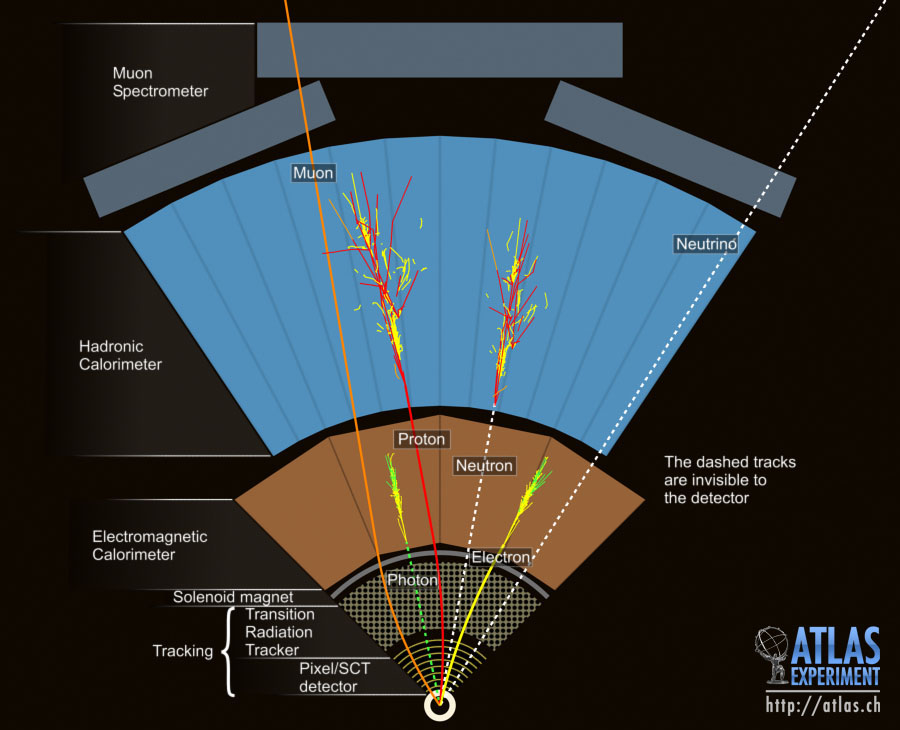
\includegraphics[width=0.7\textwidth]{schematic.jpg}
\label{fig:detector:schematic}
\caption{A schematic diagram of the interactions of various particles with detector components. Copyright CERN.}
\end{figure}

%%%%%%%%%%%%%%%% 

General purpose particle detectors thus demand the following characteristics: 

\begin{enumerate}
	\item Tracking systems must be able to identify primary and secondary vertices, while minimizing the radiation lengths before the calorimeters
	\item Strong calorimetry systems are required to accurately measure the energy and position electrons, photons, and hadrons
	\item Muon systems must be able to precisely reconstruct muons
	\item All detector systems must be capable of being read out quickly, and a triggering system is required to quickly identify interesting events for recording
\end{enumerate}

To this end, the ATLAS detector is built in the traditional onion-layer configuration, which measures particles as they travel perpendicular to the beam~\cite{ATLASPaper}. The Inner Detector, composed of the concentric Pixel, silicon microstrip (SCT), and Transition-Radiation-Tracker (TRT) subsystems, lies at the center of the detector and precisely measures tracks created by charged particles: these tracks can be used to identify the point of collision, and measure semi-long-lived particles whose decays are displaced from this origin. A 2 T solenoid encloses the Inner Detector, bending charged particles and enabling the measurement of their momenta. Next the Electromagnetic Calorimeter (ECal), composed of liquid argon (LAr) and copper, sits outside of the solenoid in a liquid nitrogen cryostat, and measures energy deposits from electrons and photons (as well as hadrons to a lesser extent). The Hadronic Calorimeter, built to measure and stop any remaining hadronic particles, is composed of steel and scintillating tile in the center (referred to as the barrel), and LAr and copper in forward regions (referred to as end-caps). Surrounding these are an additional set of magnets: the superconducting air-core toroids of the barrel and endcaps, which bend particles in the plane perpendicular to that of the bending due to the solenoid. The Muon Spectrometer (composed of monitored drift tube (MDT), resistive plate chamber (RPC), thin gap chamber (TGC), and cathode strip chamber (CSC) subsystems) sits outside of (and next to) these magnets, and provides a final measurement of the charged particles which reach that far. The entire detector is shown in Figure~\ref{fig:detector:atlas}. The incredible size of the detector--- 25 m in diameter, and 46 m long--- is dominated by the Muon Spectrometer and the toroids. On the other hand, the detector is comparatively light (only 7000 tons, compared to 14,000 tons for CMS), as the air-core toroids do not add substantial weight to the detector~\cite{CMSPaper,ATLASPaper}.


%%%%%%%%%%%%%%%%

\begin{figure}
\centering
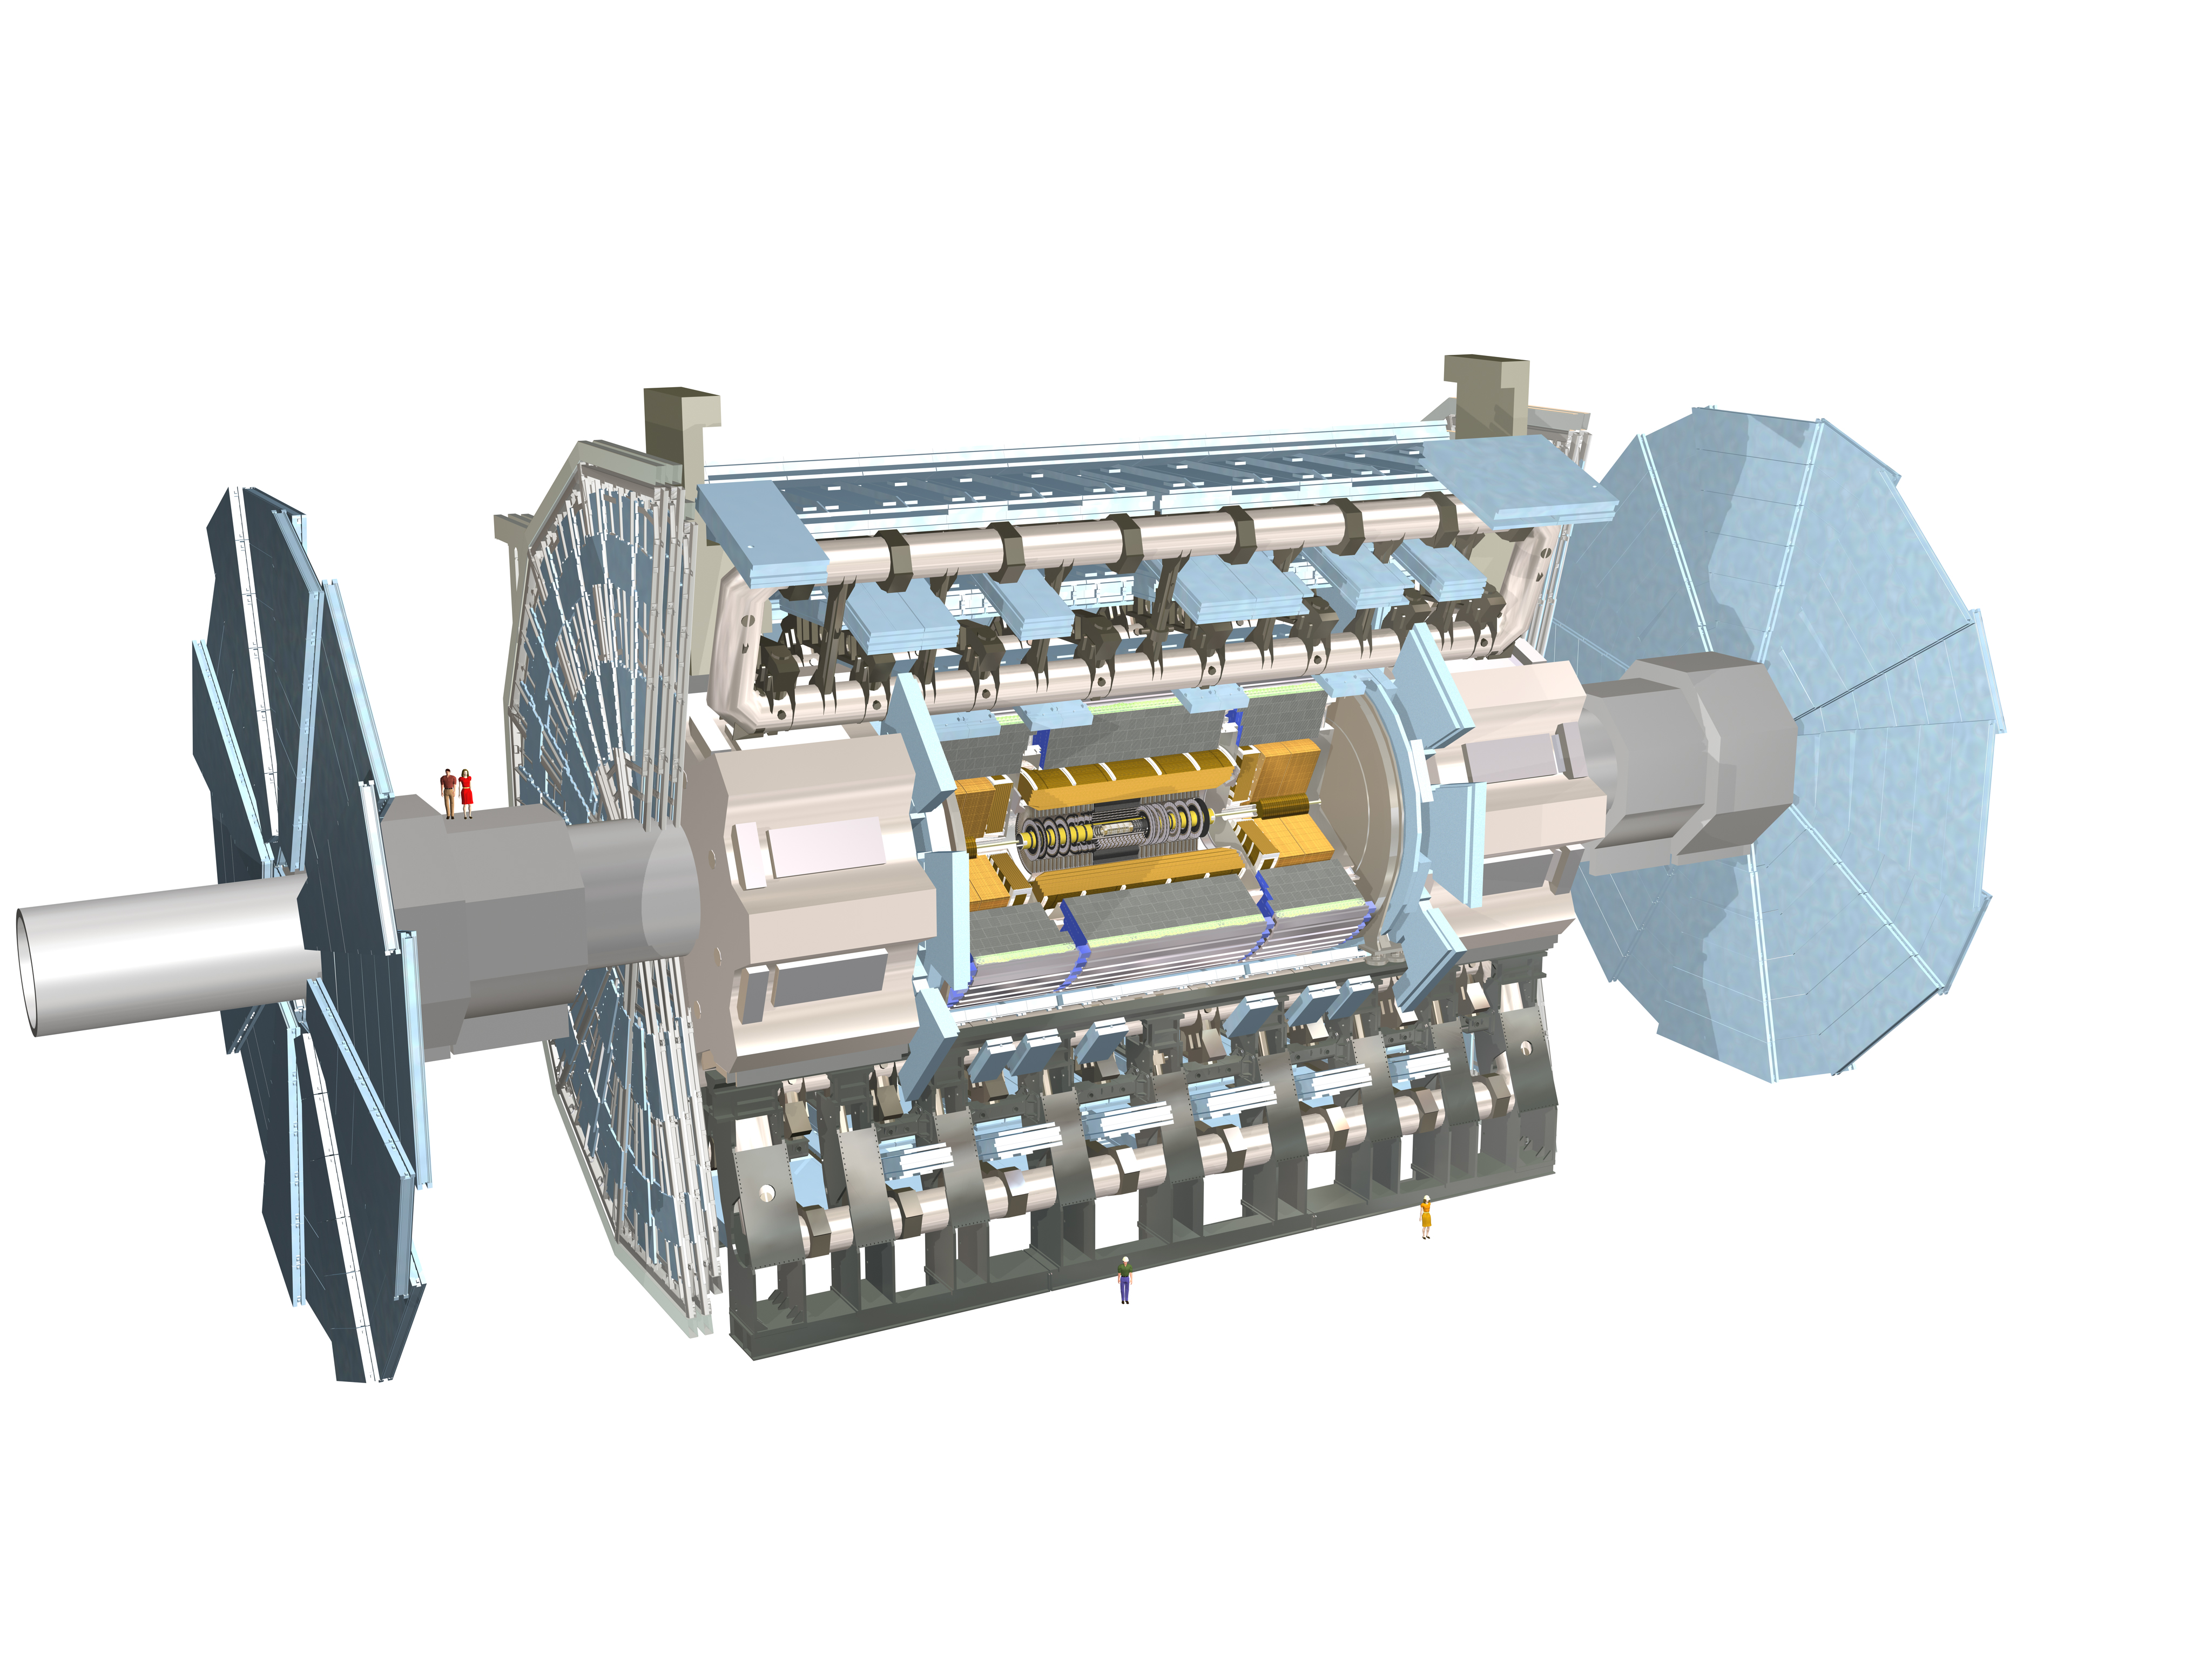
\includegraphics[width=0.75\textwidth]{atlas.jpg}
\label{fig:detector:atlas}
\caption{A computer-generated view of the ATLAS detector, with people for scale. Copyright CERN.}
\end{figure}

%%%%%%%%%%%%%%%% 


In keeping with the principle of ``similar, but opposite'' established by their locations, the ATLAS and CMS detectors take complementary approaches to the various aspects of event reconstruction in collisions. All general purpose detectors have the same basic goals, and so do ATLAS and CMS: the must reconstruct the outgoing, stable particles produced in collisions and the subsequent decays of particles in these collisions. Various particles are detected with different general classes of detectors, of which there are many possible types. For example, electrons and photons are measured by the ECal, for which ATLAS used a liquid argon and copper system while CMS used a crystal lead tungstate system. Each had their own advantages and disadvantages (ATLAS's was less costly and already proven technology with better position resolution, while CMS took a riskier route which promised better energy resolution), but overall performance between the detectors tends to be very similar because of various trade-offs. In the case of the ECals, the precision of ATLAS and CMS's $H\rightarrow \gamma \gamma$ measurements ended up being largely similar \editnote{cite higgs combination}, in no small part because CMS's all-silicon tracking system introduced greater radiation lengths before the calorimeters, thereby prompting more photons to convert and losing precision in the measurement. On the other hand, CMS's comparatively weak brass hadronic calorimeter (compared to ATLAS's higher resolution and longitudinally segmented tile calorimeter), is compensated by their tracking system, which enables a particle-flow reconstruction algorithm to combine information from all detectors and improve jet performance to levels very similar to ATLAS. \editnote{consider citations on particle flow}. Similarly, the large size and extra toroid magnets of ATLAS allow for a larger lever-arm and an additional set of measurements of muons (enabling reconstruction with or without the inner detector): however, muon reconstruction performance in CMS is very similar because the stronger solenoidal magnetic field (4 T compared to 2 T) allows for a better measurement using the inner detector only (with the muon systems on CMS providing only a tag of a passing muon, and not a complete standalone reconstruction). 


%2012 luminosity figure? Or in LHC section?

The following sections describe first the history of the ATLAS detector, and then give a detailed description of each detector subsystem. This is written from the perspective of a student who has seen the actual ATLAS detector only once, but who maintains a tremendous respect for the physicists who constructed so tremendous and beautiful a device.

%Detector figure

\section{History}

The first public discussion of the proposals which became the ATLAS detector occurred in 1992 at the General Meeting on LHC Physics at Evian-les-Bains~\cite{Evian,EvianCourier}. At the time, four general purpose detectors (much like the four detector configuration in place at LEP) were seriously considered: EAGLE, ASCOT, CMS, and L3 (as an upgrade to the existing LEP detector, including a movable stage which would allow it to take data from both $e^+/e^-$ and $pp$ collisions). Several additional single purpose (heavy ion, neutrino, and $B$-physics) detectors were also proposed.

ATLAS emerged in a later 1992 Letter of Intent as a merger of the ASCOT and EAGLE collaborations~\cite{ATLAS-LoI}. ASCOT (Apparatus with SuperCOnducting Toroids) contributed the physically-defining feature of the secondary toroidal magnet system and standalone muon measurement system, as well as the tradition of using a tortured amalgamation of letters to form a name. EAGLE (Experiment for Accurate Gamma, Lepton and Energy measurements), on the other hand, featured a stronger 2 T magnetic field and inner-detector and calorimeter designs more similar to some of the final ATLAS systems. The detector described in the Letter of Intent already resembled ATLAS in many important ways, featuring the superconducting air-core toroids, accordion-shaped liquid argon electromagnetic calorimeters, scintillating tile hadron calorimeters, and multi-design inner detector. Figure \ref{fig:detector:earlyatlas} shows an early drawing of ATLAS from the Letter, and already the detector looks recognizable to its current form.

% Any citations on UA1 origins?

%%%%%%%%%%%%%%%%

\begin{figure}
\centering
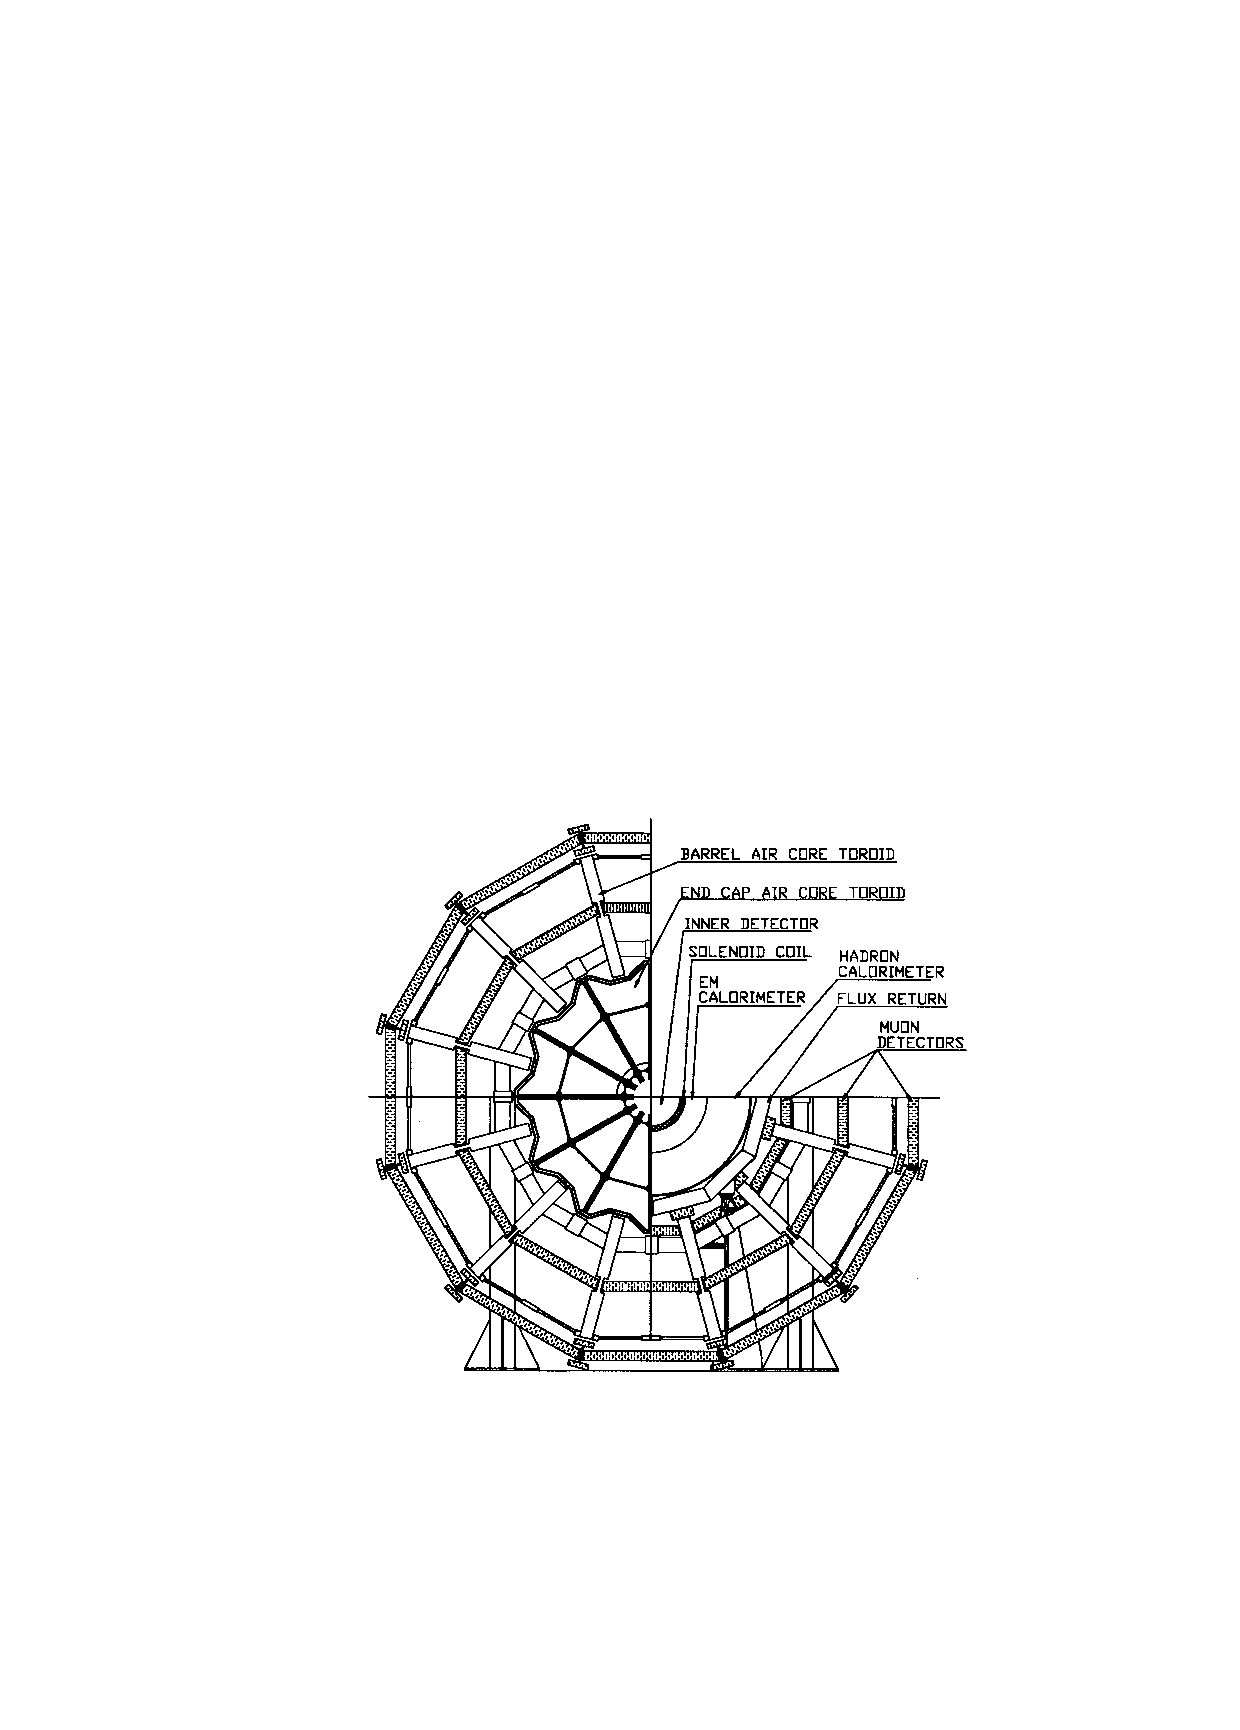
\includegraphics[width=0.7\textwidth]{early-atlas.pdf}
\label{fig:detector:earlyatlas}
\caption{An early view of a potential superconducting air-core toroid magnet system for the ATLAS detector from the 1992 Letter of Intent~\cite{ATLAS-LoI}.}
\end{figure}

%%%%%%%%%%%%%%%% 

By the release of the 1994 Technical Proposal~\cite{ATLASTP}, the detector design was becoming much more complete, and many of the choices of design for the detector subsystems (the components of the ID, for example) were already mostly complete. This year also saw the American institutions joining the collaboration (Brookhaven and Columbia University), and the refugees from the demise of the SSC would continue to rapidly join ATLAS in the coming years. \editnote{find a citation for this? usatlas?} By 1997 many of the detector subsystem Technical Design Reports (TDR) were complete, and construction began on these systems~\cite{ATLASHistory}. 1999 saw a TDR for the entire detector, representing a complete integrated design for the entire detector~\cite{tdr1,tdr2}. Memoranda of Understanding with national funding institutions are completely arranged by 2000, as construction of the detector was well underway~\cite{ATLASHistory}. The cavern, the largest yet built at CERN and pictured in Figure~\ref{fig:detector:cavern}, was completed in 2003. Assembly of detector components continued rapidly at this point, and the detector was finished in 2008.

%%%%%%%%%%%%%%%%

\begin{figure}
\centering
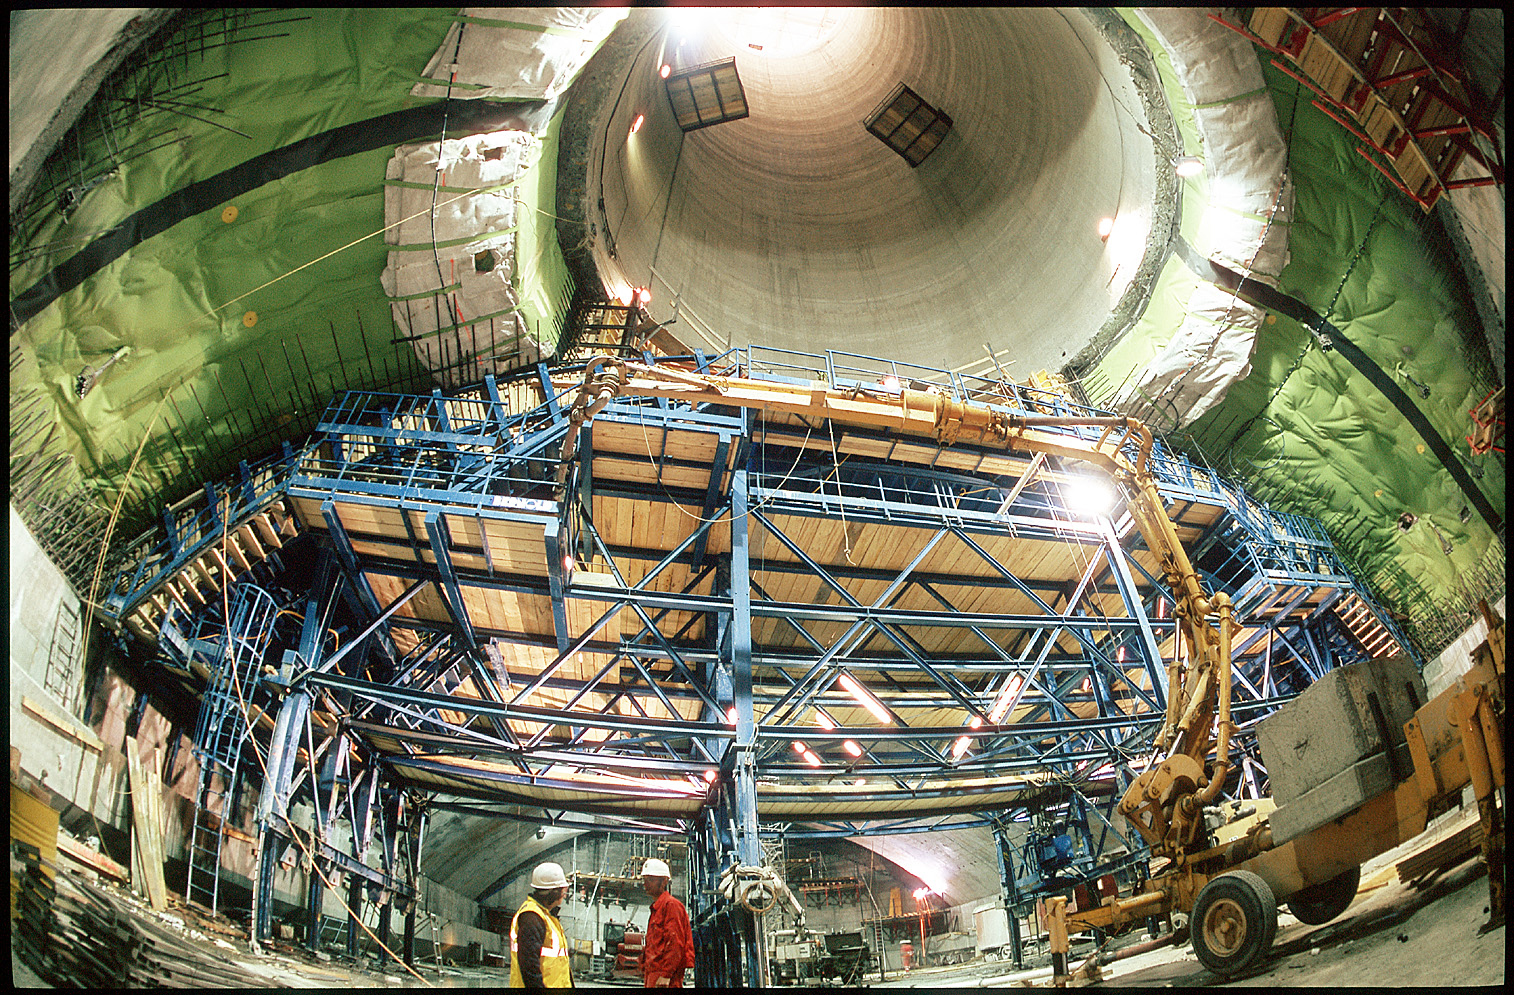
\includegraphics[width=0.7\textwidth]{cavern.jpg}
\label{fig:detector:cavern}
\caption{A view of the ATLAS cavern during construction. Copyright CERN.}
\end{figure}

%%%%%%%%%%%%%%%% 

Early data-taking was of course disrupted by the incident described in Section~\ref{lhc:history}, and first 7 TeV collisions were recorded on March 3, 2010. ATLAS recorded 35 \ipb~in 2010, 4.6 \ifb~in 2011, and 20.3 \ifb~in 2012. The dramatic increase of data during 2011 and 2012 came at the cost of pileup levels far higher than what had been planned for. As Section~\ref{atlas:data-quality} describes, the detector operated incredibly well during these difficult conditions, and over 90\% of data delivered by the LHC was successfully recorded.





% approval dates

% cavern construction (picture?)

% construction milestones

% first data, first papers

% quenching? higgs discovery


\section{Magnet Systems}

The magnets of ATLAS play a critical role in the meausurement of particle momenta by bending charged particles via the interaction with the Lorentz Force Law:

\begin{equation}
\frac{d \vec{p}}{d t} = q (\vec{E} + \vec{v} \times \vec{B})
\end{equation}
%
where $\vec{p}$ is the particle 4-momentum, $q$ is the charge, $v$ is the velocity, and $E$ and $B$ are the electric and magnetic fields. The solenoid, for example, has a field in $z$ direction only, resulting in a force in the $\phi$ direction. As the magnetic field does no work, the energy of the particle is not changed, and only the direction is affected. The degree of bending is directly proportional to $\vec{v}$, the velocity, and so the particle's momentum is able to be extracted. The field configuration in the toroid systems is much more complicated, but the particle momentum reconstruction follows the same general principle. While the magnetic field in the toroids is not constant, and therefore the direction of bending is more complicated than in the solenoid, the goal is to bend the particles in a direction perpendicular to that of solenoid: this allows for a completely independent measurement of the track's trajectory, with no bias from the original measurement. \editnote{Cite.}

The combined magnet system is shown in Figure~\ref{fig:detector:magnets}. The solenoid sits at the center, and the toroid system on the outside and in the endcaps.

%%%%%%%%%%%%%%%%

\begin{figure}
\centering
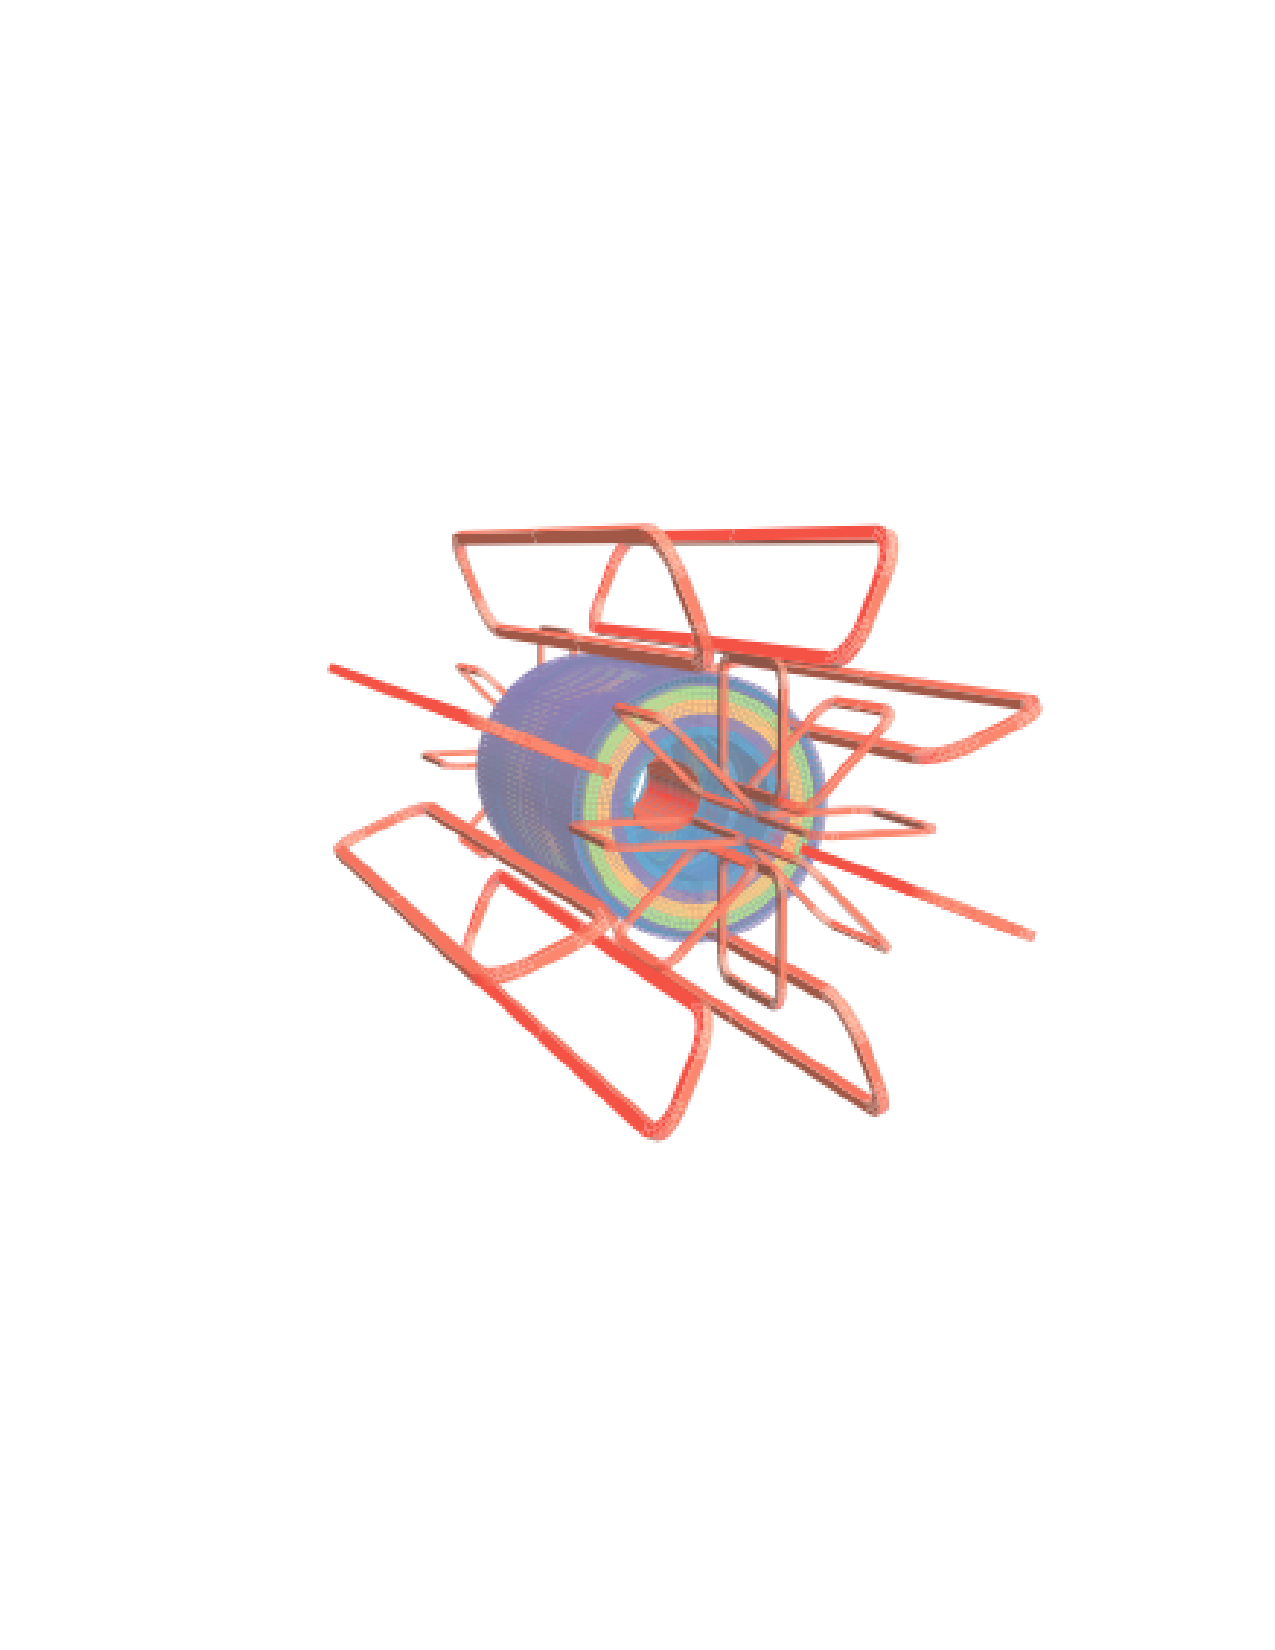
\includegraphics[width=0.65\textwidth]{magnet-fields.pdf}
\label{fig:detector:magnets}
\caption{A computer generated visualization of the ATLAS magnet systems.}
\end{figure}

%%%%%%%%%%%%%%%% 


\subsection{Solenoid}
\label{atlas:magnets:solenoid}

ATLAS's solenoid is shown in Figure~\ref{fig:detector:solenoid} shortly after its construction was finished. It sits inside the calorimeter systems, and surrounds the Inner Detector. This is contrast to the configuration in CMS, where the solenoid surrounds the calorimeter systems. Thus, particles in ATLAS do not bend in the calorimeters and particle showers tend to be more directly collimated, while particles tend to be dispersed much further in the calorimeter in CMS.

The ATLAS solenoid has a 2 T axial field, powered by 7.730 kA of current~\cite{ATLASPaper}. Since the solenoid is in front of the calorimeters, care must be taken to reduce the material that particles can interact with. To that end, the magnet and the LAr calorimeter share the same vacuum vessel, eliminating the need for two additional walls. The magnet is composed of Al-stabilized NbTi conductor, developed specifically to best balance high field and low material length. The solenoid occupies the space between 2.46 and 2.56 m, and is 5.8 m long axially. The stored energy of the magnet system is approximately 40 MJ, and it takes approximately a week to cool the magnet to the operational temperature of 4.5 K. 

%%%%%%%%%%%%%%%%

\begin{figure}
\centering
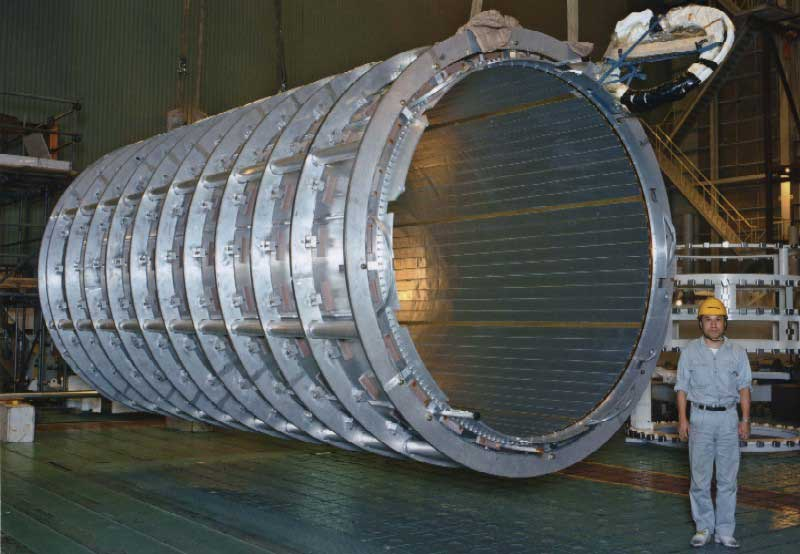
\includegraphics[width=0.7\textwidth]{solenoid.jpg}
\label{fig:detector:solenoid}
\caption{A photograph of the ATLAS solenoid shortly after the winding of the coils was finished. Copyright CERN.}
\end{figure}

%%%%%%%%%%%%%%%% 


\subsection{Barrel toroids}

The ATLAS magnet system contains two separate toroids systems~\cite{ATLASPaper}. The barrel toroid consists of 8 coils in separate racetrack-configured, stainless-steel vacuum vessels which give the ATLAS the detector its famous shape, as seen in Figure~\ref{fig:detector:toroid}. The magnets are supported by a system of 8 inner and 8 outer support rings. The entire system is 25.3 m long, and begins at 9.4 m radially and ends at 20.1 m. The magnet is composed of the same wire as used in the solenoid, and the magnet system stores 1.1 GJ of energy during operation at 20.5 kA of current. The barrel toroid takes approximately 5 weeks to cool to its nominal temperature of 4.6 K.


%%%%%%%%%%%%%%%%

\begin{figure}
\centering
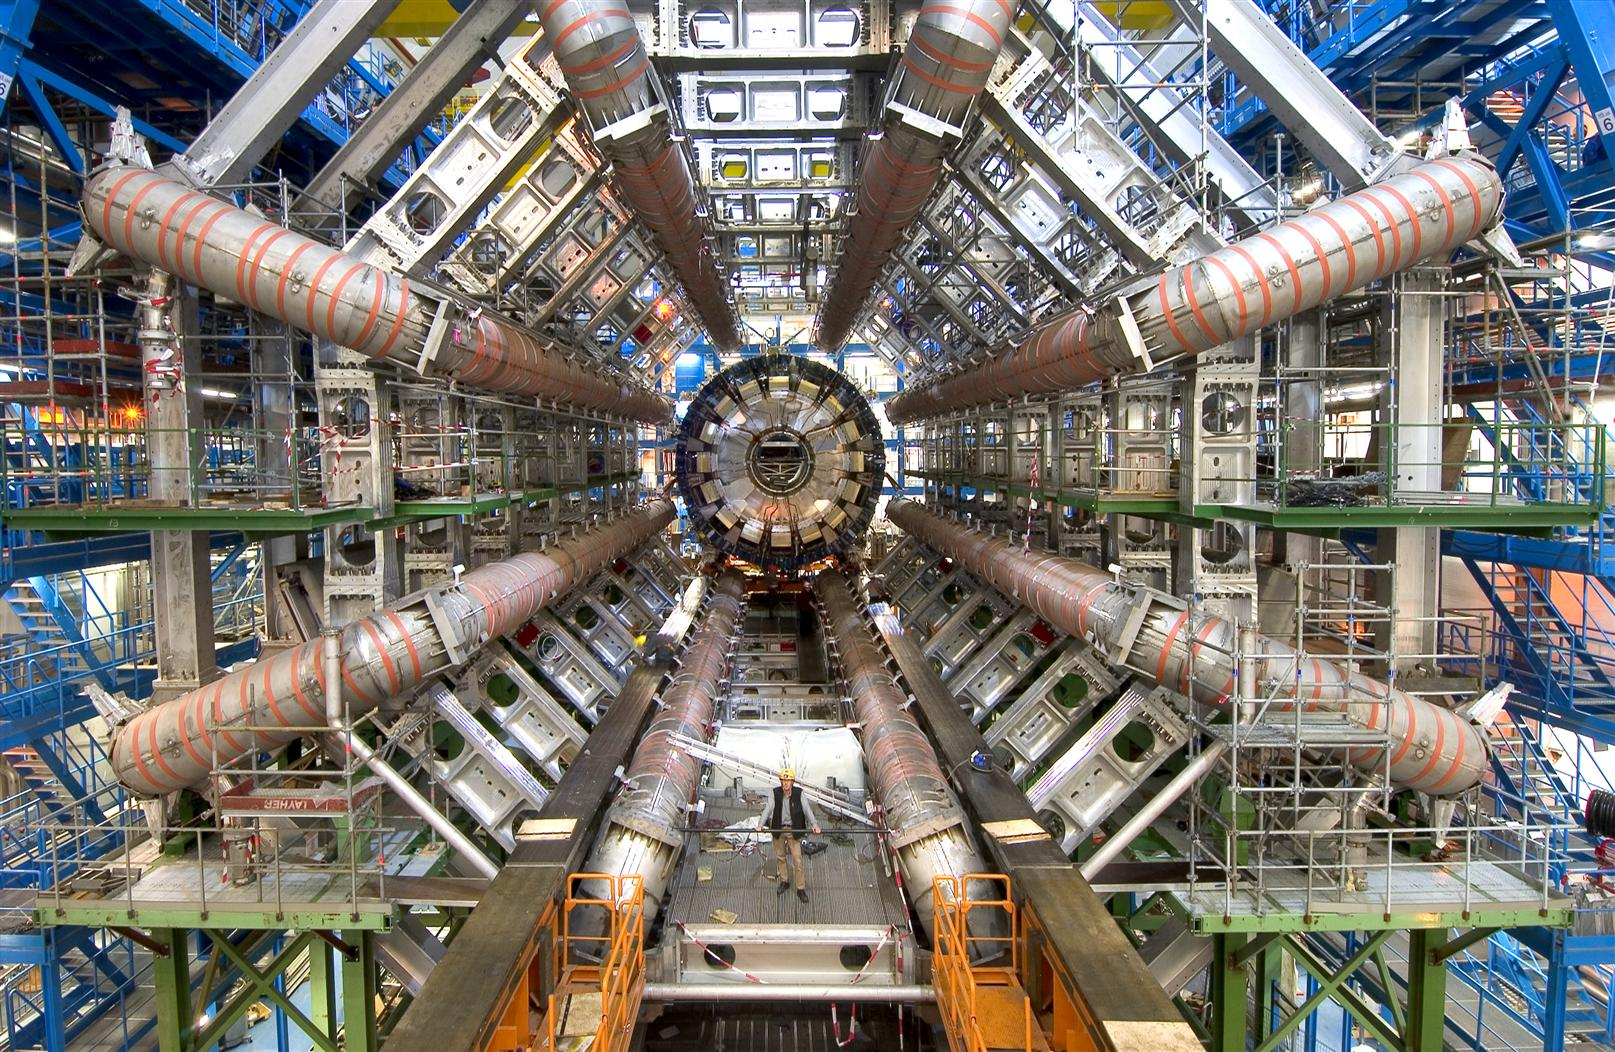
\includegraphics[width=0.7\textwidth]{toroid.jpg}
\label{fig:detector:toroid}
\caption{A photograph of the ATLAS barrel toroids after their installation. Note person in the center for scale. Copyright CERN.}
\end{figure}

%%%%%%%%%%%%%%%% 

\subsection{Endcap toroids}

The third ATLAS magnet system are the endcap toroids~\cite{ATLASPaper}. These magnets are designed bend the muons which interact with the muon spectrometer endcaps. They are constructed to be removable in order to allow access to the calorimeter and inner detector systems. The endcaps are each constructed of 8 flat, square coils with 8 keystone wedges which share the same cryostat. The magnets each take four weeks to cool to the operating temperature of 4.5 K, and operate at 20.5 kA with a stored energy of 0.25 MJ each. The coil material is again largely similar to that of the barrel toroid and solenoid. One of the endcap toroids is pictured in Figure~\ref{fig:detector:endcap-toroid} after being lowered into the ATLAS cavern.


%%%%%%%%%%%%%%%%

\begin{figure}
\centering
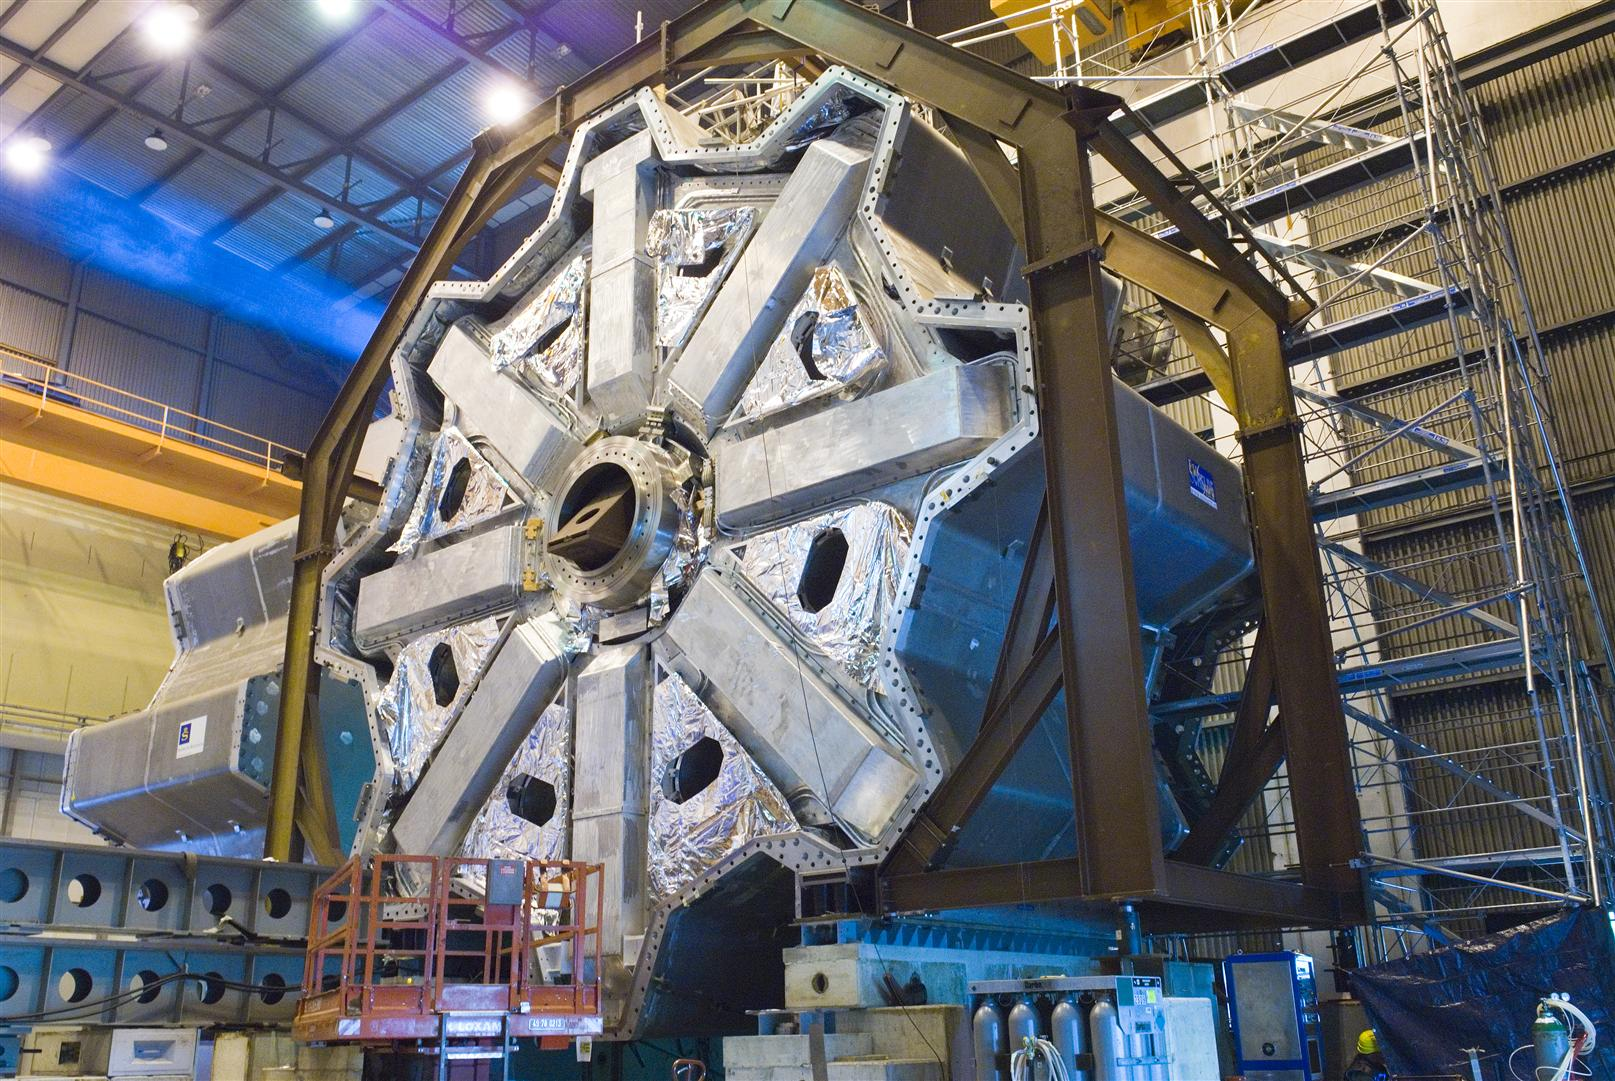
\includegraphics[width=0.7\textwidth]{endcap-toroid.jpg}
\label{fig:detector:endcap-toroid}
\caption{A photograph of an ATLAS endcap toroid shortly before its installation in the detector. Copyright CERN.}
\end{figure}

%%%%%%%%%%%%%%%% 


\section{Inner Detector}

The ATLAS Inner Detector (ID) sits at the center of the experiment~\cite{ATLASPaper}. The purpose of the detector is to reconstruct the tracks (i.e. trajectories) of charged particles produced by the collisions of the LHC in order to not only accurately measure the locations of collisions and particle decays, but to also directly measure the momenta and locations of charged particles~\cite{ATLASExpected}. Tracks, discussed more in depth in Section~\ref{tracking}, are lines drawn between several independent measurements in different layers of the detector: each individual measurement is a snapshot of the particle's trajectory out from the collision point, and dedicated tracking algorithms are used to combine these snapshots to extract the desired information.

The detector covers the range $|\eta| < 2.5$, and is capable of measuring particle momenta as low as $\pT = 500$~MeV. Charged particle reconstruction efficiencies are typically greater than $90\%$ for 100 GeV particles and $70\%$ for 1 GeV particles, with a large $\eta$ dependence. Typical \pT resolutions are of order $0.05\% \mathrm{GeV}^{-1} \times \pT \oplus 1\%$, and impact parameter resolutions are approximately 10 $\mu$m\footnote{The impact parameter is the perpendicular distance from the origin to the point of closest approach of the track, and is critical for the measurement of secondary vertices.}. 

The ID is composed of several independent detector subsystem which read out the locations of interactions with charged particles. These hits are fit to tracks by a suite of tools, which include standard global-$\chi^2$ and Kalman-filters, but also several specialized fitters~\cite{ATLASExpected}. The \pT of the particles is obtained by measuring the curvature produced by the 2 T solenoid (as described by Section~\ref{atlas:magnets:solenoid}) surrounding the detector. The three subsystems, described below, are the silicon pixel tracker (Pixel), silicon microstrip tracker (SCT), and transition radiation tracker (TRT). The combined detector has a length of 7024 m and a radius of 1.15 m~\cite{ATLASPaper}. Figure~\ref{fig:detector:inner-detector} shows a computer generated image of the combined ID, and Figure~\ref{fig:detector:inner-detector-2} shows a computer-generated image of the various subcomponents of the ID and their spacing. Figure~\ref{fig:detector:inner-detector-3} shows the $\eta$ range of the various detector subsystems, displaying the transition between barrel and endcap components.


At design luminosity, the detector is expected to measure approximately 1000 charged particles every 25 ns within the detector acceptance~\cite{ATLASExpected}. The added growth of pileup in the 2012 and future LHC runs have increased the importance of the Inner Detector as the primary vertex identification has become even more critical~\cite{ATLAS-CONF-2012-042}, but growing challenges from the computing time necessary to fit so many tracks (which increase more than quadratically as the number of detector hits~\cite{Combinatorics}) will also need to be overcome to make best use of the detector's information.

%%%%%%%%%%%%%%%%

\begin{figure}
\centering
\includegraphics[width=0.7\textwidth]{inner-detector.jpg}
\label{fig:detector:inner-detector}
\caption{A computer-generated view of the ATLAS inner detector, with relevant sizes of the detector marked out. Copyright CERN.}
\end{figure}

%%%%%%%%%%%%%%%% 

%%%%%%%%%%%%%%%%

\begin{figure}
\centering
\includegraphics[width=0.7\textwidth]{inner-detector-2.jpg}
\label{fig:detector:inner-detector-2}
\caption{A cut-out view of the ATLAS inner detector, showing the layers a particle would interact with as it passed outward from the collision point. Copyright CERN.}
\end{figure}

%%%%%%%%%%%%%%%% 

%%%%%%%%%%%%%%%%

\begin{figure}
\centering
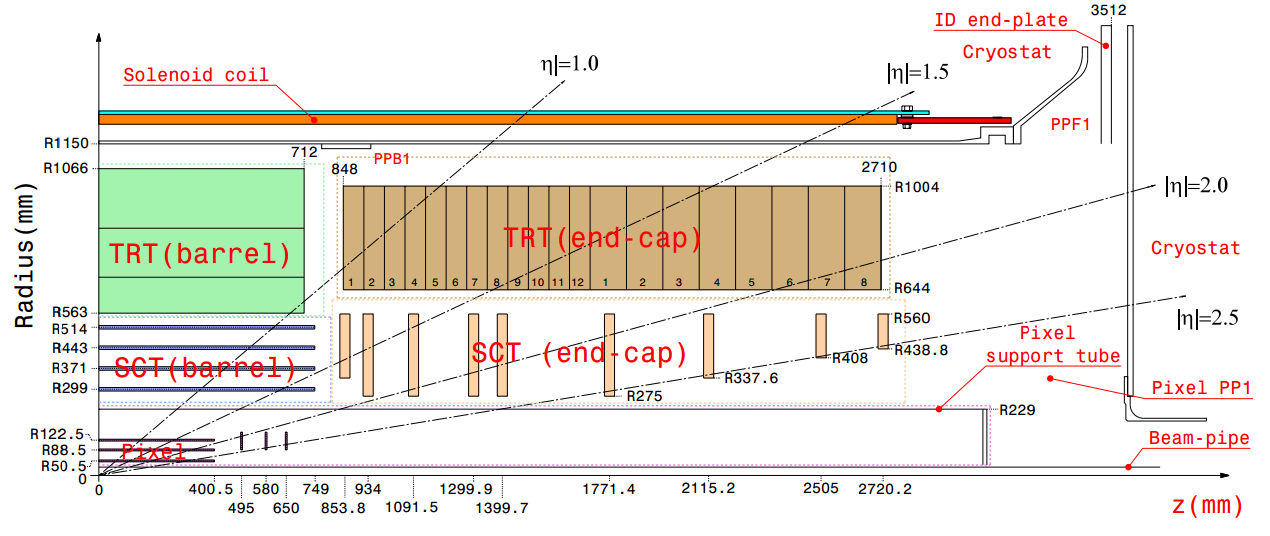
\includegraphics[width=0.7\textwidth]{tracker-eta.png}
\label{fig:detector:inner-detector-3}
\caption{A cut-out view of the Inner Detector and the locations in $r$, $z$ (with lines of detector $\eta$ demarcated) of the various detector subsystems.}
\end{figure}

%%%%%%%%%%%%%%%% 


\subsection{Silicon Pixel Detector}

The innermost ATLAS sub-detector is the Silicon Pixel Detector~\cite{Pixel,ATLASPaper}. The principal of detection for the pixel detector follows the standard ionizing radiation detector~\cite{Detectors}. Charged particles interact with the active medium (doped silicon), knocking electrons loose from their host atoms and creating electron-hole pairs. An applied voltage carries the holes and electrons to opposite ends of the detectors, where they are read out. The active regions are very small in both $x$ and $y$ dimensions, allowing for many independent measurement channels in a small area. Given the high number of particles expected from LHC collisions, and that the density is greatest nearest to the interaction point, it is critical that the innermost detector have a huge number of very small channels, making the task perfectly suited for a pixel detector.

80.4 million independent pixel channels, with a size of $50 \times 400~\mu$m, are read out by 1744 bump-bonded modules attached to the active sensors. Each of the modules are composed of 16 radiation hard front-end chips~\cite{ATLASPaper}. This corresponds to a combined active area of 1.7 $m^2$. The detector is arranged in three radial layers in the barrel section, and three disks in the end-caps. In the radial layers, the pixels have a resolution of $10 \times 115~\mu$m in $R-\phi$ and $z$ respectively, and in the end-caps the orientation is perpendicular and the resolution is $10 \times 115~\mu$m in $R$ and $R-\phi$: the orientations are always chosen such that the most precise measurement takes place in the direction most relevant to the measurement of the track $p_T$.\footnote{The $R-\phi$ coordinate is simply a distance-projected version of the azimuthal angle $\phi$.} The barrel and disk arrangement is shown in Figure~\ref{fig:detector:pixel}. Hits are read out when charge has been collected over a tunable threshold determined by the noise of each pixel, resulting in typical occupancies of $10^{-4}$ -- $10^{-5}$, though this grows obviously grows with additional $pp$ interactions.

The innermost radial layer, known as the $b$-layer, sits only 50.5 mm from the center of the beampipe, while the outermost layer is located at 122.5 mm~\cite{ATLASPaper}. By placing detectors so close to the interaction point, it is possible to very accurately measure the location of both  primary vertices--- the locations of $pp$ collisions--- and second vertices-- the locations of the displaced decays of particles with long lifetimes, such as $B$-hadrons~\cite{ATLASExpected}.

Placing the detector so close to the beamline comes at a price, however, as the detector is particularly susceptible to radiation damage due to the high flux of particles through a small area. At design luminosity, this is expected to be about 158 kGy/year at the $b$-layer, reduced to 25.4 kGy/year at the outermost layer~\cite{ATLASPaper}. Damage comes in the form of displaced atoms in the doped silicon lattice, resulting in lower electron-hole yields per particle interaction. Some of the damage is mitigated by operating at cold temperatures (typically $-5$ to $-10$\degree~C), and higher bias voltages can also alleviate the effects.

While the entire Inner Detector is expected to be replaced after 300 \ifb~are collected in order to replace the damaged components, the long shutdown of 2013-2015 presented ATLAS with the opportunity to augment the existing pixel detector with the so-called Insertable B-Layer (or IBL)~\cite{ATLASIBL}. The IBL, which adds an additional layer of pixels to the barrel and endcap pixel systems, is attached directly to a new carbon-fiber beampipe, and is located only 33 mm from the center of the beampipe. Due to this extremely close distance, the pixel size has been further reduced to $50 \times 250 \mu$m. The vertexing performance (especially secondary vertex identification for $b$-tagging) of ATLAS in Run 2, starting in 2015, is expected to substantially increase due to the IBL. 

%%%%%%%%%%%%%%%%

\begin{figure}
\centering
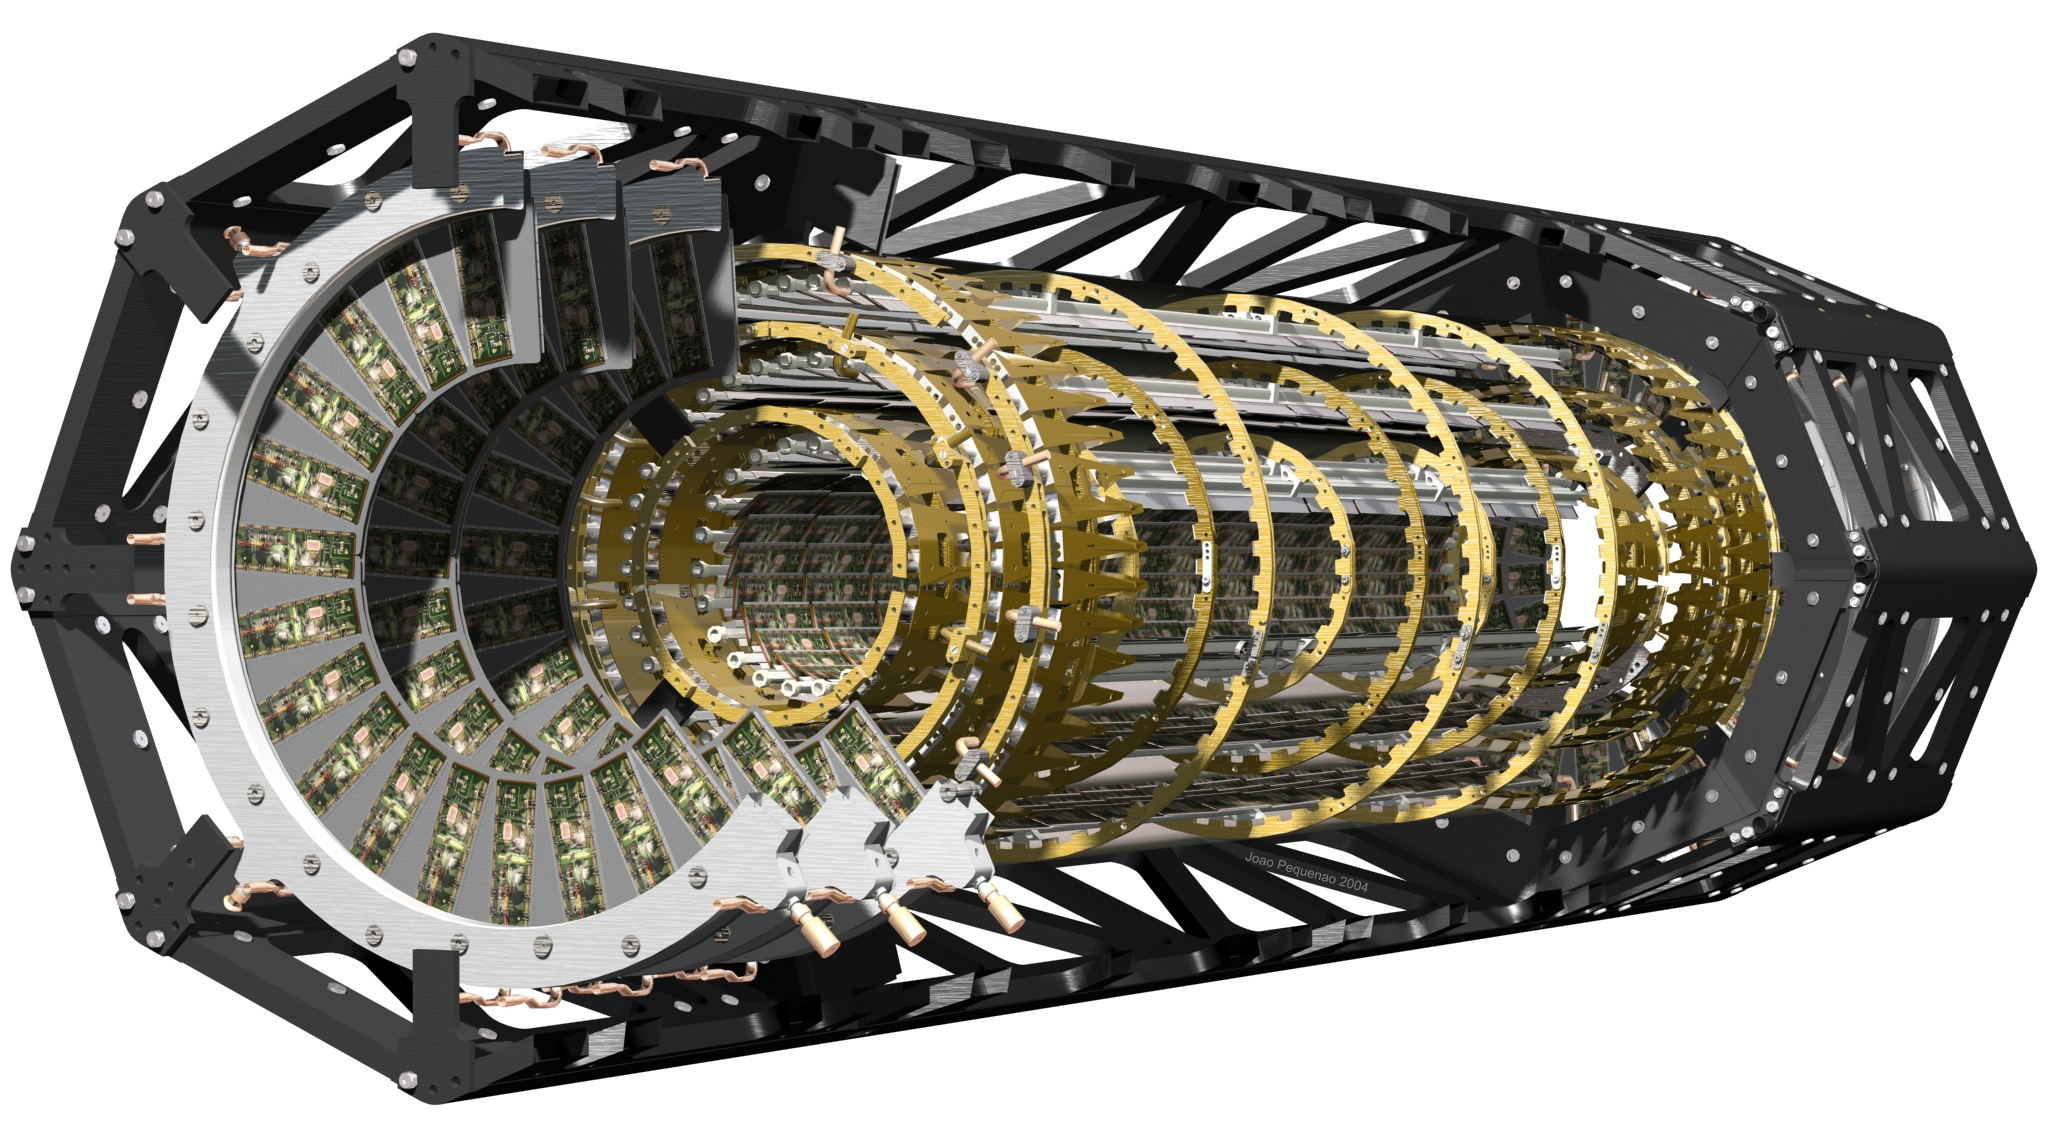
\includegraphics[width=0.7\textwidth]{pixel.jpg}
\label{fig:detector:pixel}
\caption{A computer-generated view of the ATLAS pixel detector. Copyright CERN.}
\end{figure}

%%%%%%%%%%%%%%%% 



\subsection{Silicon Strip Tracker}

The next outermost subdetector in the ID is composed of silicon microstrip layers~\cite{SCTPaper,ATLASPaper}, and is commonly referred to as the SCT.  The SCT operates under a very similar principal to the Pixel detector: doped silicon under an electric bias is the active medium, and electron/hole pairs are collected to read out hits. Unlike the Pixels, one dimension of the detector is ganged together to form the eponymous strips. Two sets of detectors must therefore placed perpendicularly to each other (or at some other angle) to provide a true two-dimensional spatial measurement, but the number of channels to be read out has been significantly reduced~\cite{Detectors}.

The ATLAS SCT contains 4088 modules, each composed of two 64 mm silicon strip sensors with a 40-mrad angular offset~\cite{ATLASPaper}. Like the Pixels, the detector is arranged into radial layers in the barrel and disks in the endcap, of which there are 4 and 9 respectively. The strips have a resolution of $17 \times 580$ in $R-\phi$ and $z$ respectively in the barrel, and $17 \times 580$ in $R-\phi$ and $R$ in the disks. The SCT occupies the space between 275 mm and 560 mm from the beamline. The detector contains a total of 6.3 million read out channels read out by radiation hard front-end chips~\cite{SCTReadout}. The increased distance of the SCT from the beamline significantly lowers the rate of expected radiation damage, but increased bias voltages are still expected to be necessary after significant luminosity~\cite{SCTPaper,ATLASPaper}.  Figure~\ref{fig:detector:sct} shows one segment of the SCT endcap disks.


%%%%%%%%%%%%%%%%

\begin{figure}
\centering
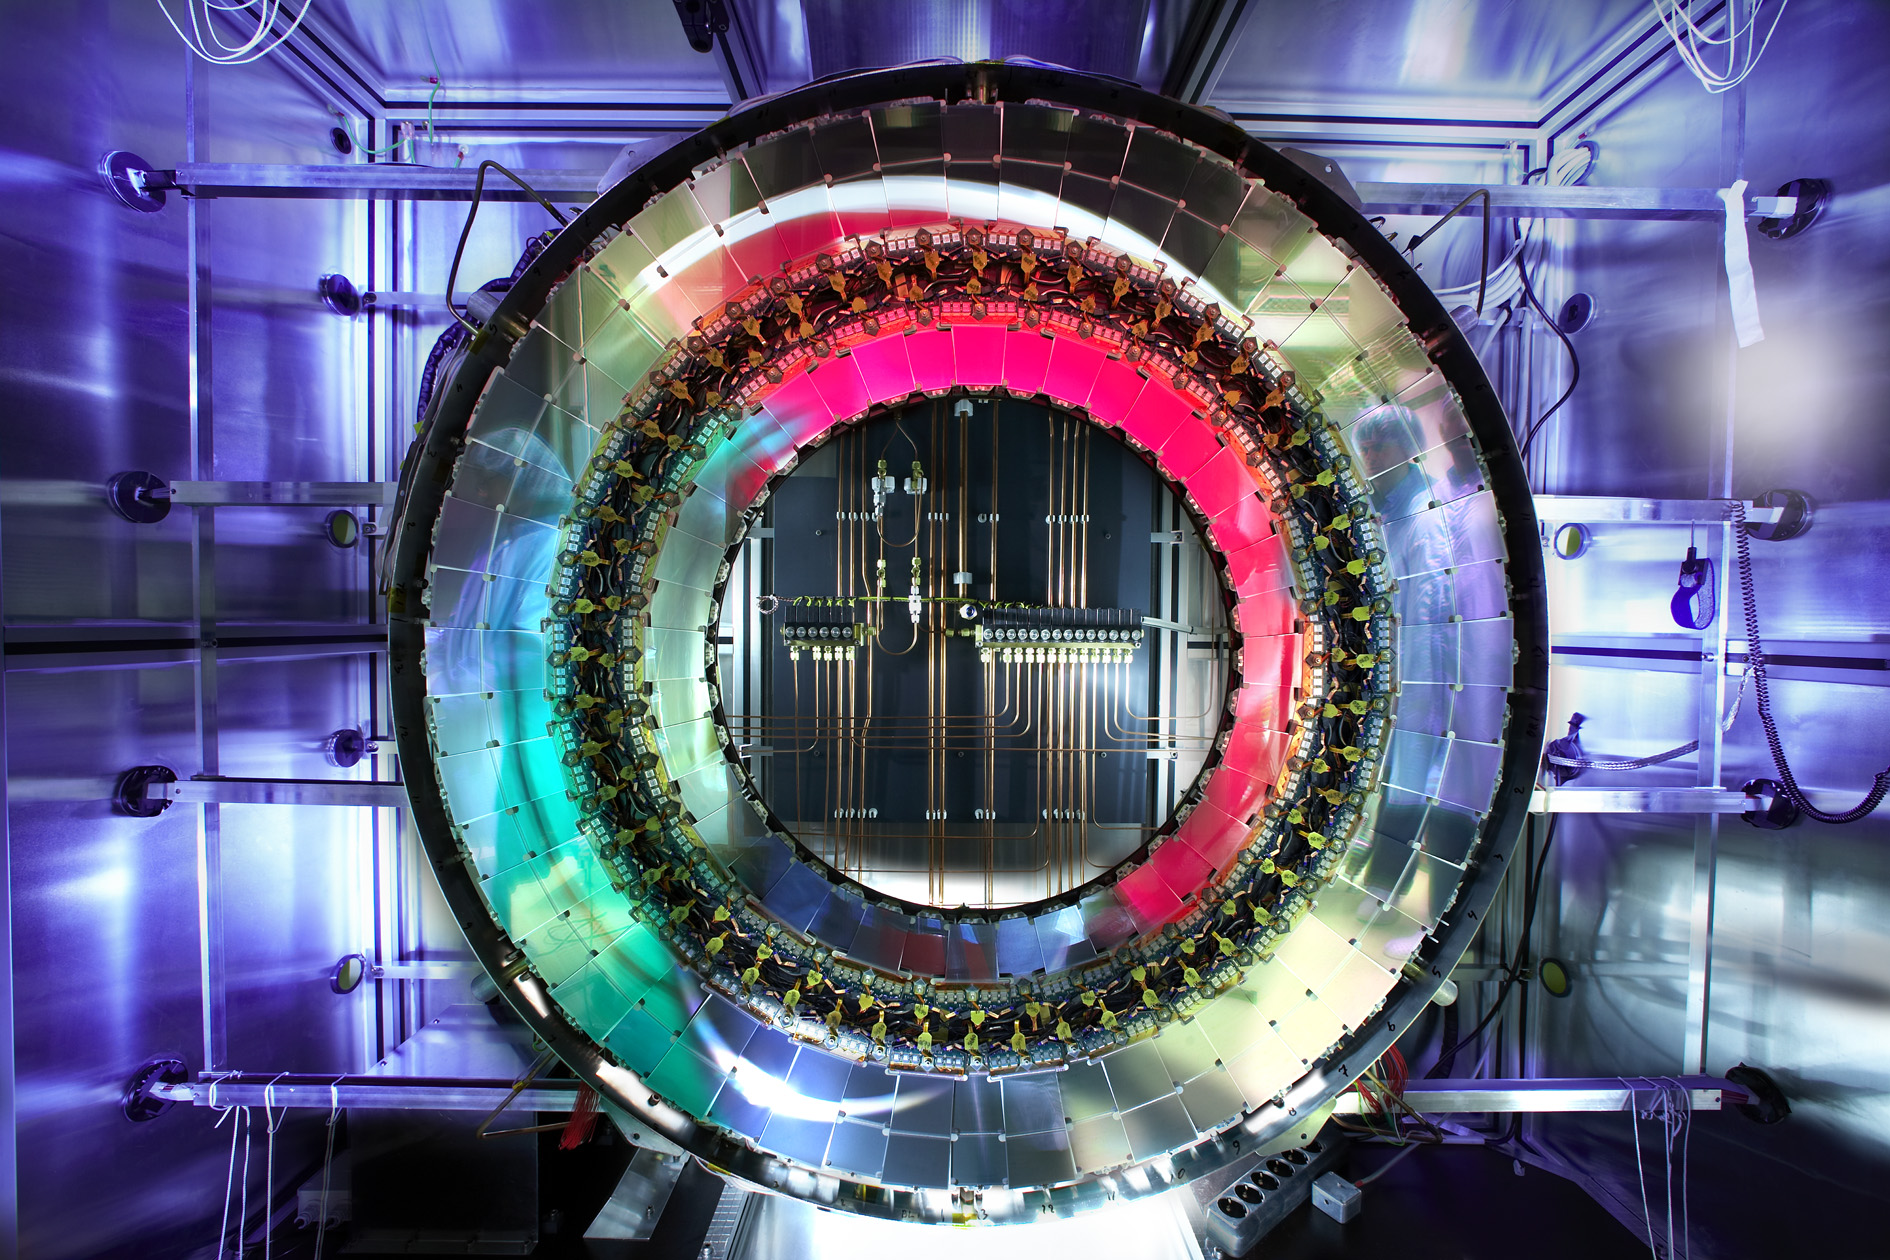
\includegraphics[width=0.7\textwidth]{sct.jpg}
\label{fig:detector:sct}
\caption{A photograph of one segment of the ATLAS SCT endcap disks. Copyright CERN.}
\end{figure}

%%%%%%%%%%%%%%%% 

\subsection{Transition Radiation Tracker}
\label{detector:ID:TRT}
The final subdetector of the ID is the transition radiation tracker~\cite{ATLASPaper}. Unlike the other subdetectors of the ID, the TRT is not made out of silicon: instead, it is composed of 2 mm (in radius) straw tubes (proportional drift tubes)~\cite{ATLASPaper}. The tubes detect particles via ionization: particles traversing the tube interact with the gas in the tube (70 $\%$ Xe, 27 \% CO$_2$, and 3 \% O$_2$) and create ion/electron pairs~\cite{Detectors,ATLASPaper}. The exterior of the tube is a cathode, and a center wire is an anode, set at a voltage difference of 1530 V. The extreme electric field in the tube accelerates the electrons rapidly through the gas, colliding with other atoms and creating more ion/electron pairs, creating an avalanche which greatly amplifies the original signal~\cite{Detectors}. The time of arrival of the signal to the anode depends on the position of the initial collision and the known drift velocity of the gas, thus allowing for an accurate radial measurement of the interaction point~\cite{TRTReadout}, but no information about the location of the interaction along the length of the tube.

The TRT covers the range $|\eta| < 2.0$ in the standard barrel and endcap arrangements~\cite{TRTPaper}. There are 52544 tubes, each 1.44 m in length, arranged in two active regions on either side of the center of the detector. The endcaps are each composed of 122880 370 mm long tubes, organized into 18 wheels. The barrel is arranged in layers of 76 straws, while the endcaps have 160 planes. There are a combined 350848 channels in the detector. Figure~\ref{fig:detector:trt} shows a photograph of the TRT barrel during testing.

The TRT, whose active elements are much larger than that of the silicon sensors in the rest of the ID, has a significantly larger hit resolution: 130 $\mu$m in $R-\phi$~\cite{ATLASPaper}. This is partly compensated by the large number of straws that charged particles cross, generating on average 30 hits~\cite{ATLASExpected}. The TRT has the added benefit of providing identification of electrons via the emission of transition X-rays~\cite{TRTPID}. X-ray photons can be emitted as a relativistic electron passes through materials with different dielectric constants; the X-rays can subsequently interact with the straw tube gas and cause an ionization with a much higher energy than for a direct hit (15 keV, compared to 2 keV)~\cite{TRTReadout}. This extra energy can be recorded and used later for identification of the electron. In the barrel, the TRT straws are embedded in a set of polypropylene-polyethylene fibers with a diameter of 19 $\mu$m; in the endcap, foil is interleaved between the straws. This type of identification is not possible with silicon detectors, providing the TRT with a unique capability. Finally, the gas tubes of the TRT present a significantly lower amount of material to particles traversing the ID compared to silicon detectors, thereby degrading less the performance of the subsequent ECal and HCal.

Given the distance of the TRT from the interaction point, and the greater resilience of gas tubes to radiation compared to silicon (there is no atomic lattice to be damaged), the TRT is not expected to be significantly damaged during the course of data-taking. However, with the presence of increasing pileup conditions in upcoming runs, the occupancy of the TRT is expected to grow significantly, presenting a significant challenge to continued operation~\cite{TRTOccupancy}.

%%%%%%%%%%%%%%%%

\begin{figure}
\centering
\includegraphics[width=0.7\textwidth]{trt.jpg}
\label{fig:detector:trt}
\caption{A photograph of the ATLAS TRT system during testing. Copyright CERN.}
\end{figure}

%%%%%%%%%%%%%%%% 

\section{Calorimeters}

The ATLAS calorimeters lie outside of the ID and the solenoid, and are responsible for a near-hermetic ($|\eta| < 4.9$) measurement of all particles except for muons and neutrinos~\cite{ATLASPaper}.  The calorimeter system is also critical in stopping particles (besides muons) from entering the muon spectrometer. The calorimeters are the primary detectors of interest in the reconstruction of hadronic events, as they are the only detectors capable of measuring neutral particles which the tracker can miss. The operation of these detectors is thus critical for both searches for new physics in hadronic channels and for measurements of hadronic phenomena in the Standard Model.

The combined calorimeter system is pictured in Figure~\ref{fig:detector:calo}. There are several subsystems: the LAr electromagnetic barrel, the tile barrel, tile extended barrel, the LAr electromagnetic endcap (EMEC), the LAr hadronic endcap (HEC), and the LAr forward calorimeter (FCal)~\cite{ATLASPaper}. The central LAr barrel also has a presampler layer, which estimates the energy lost before the particles reach the ECal.

All the detectors are non-compensating, sampling designs. Sampling detectors are designed in alternating layers of passive absorber and active readout. The passive layers are composed of some dense material (steel, lead, etc.) which, because of the high density of atoms, causes many interactions with the incoming particles, creating cascades of daughter particles. The energy of these low energy daughter particles is easier to measure than the original high energy particle, so the passive layers play an important role in the measurement. The active layers measure the energy of the showers--- via mechanisms such as scintillation or ionization--- and the process repeats several times, gradually reducing the energy of the shower with each layer and thereby stopping the particles. The non-compensating nature of the calorimeter means that energy is lost in each of these passive layers: the full energy read out by the active layers will not be that of the incoming particles. Calibrations, described in Chapter~\ref{chapter:jet-reconstruction}, can correct for the central value of this unmeasured energy, but fluctuations in the shower development inevitably mean that there is a price in terms of energy resolution~\cite{Wigmans}. The details of homogenous vs. sampling, and compensating vs. non-compensating designs depend greatly on the conditions of the collider, and the designs selected by ATLAS were chosen based on the compromises between expected performance gains and cost.\footnote{The CMS lead-tungstate crystal ECal is an example of a non-sampling device, as the same crystals promote shower growth and are read out to measure the energy.}



%%%%%%%%%%%%%%%%

\begin{figure}
\centering
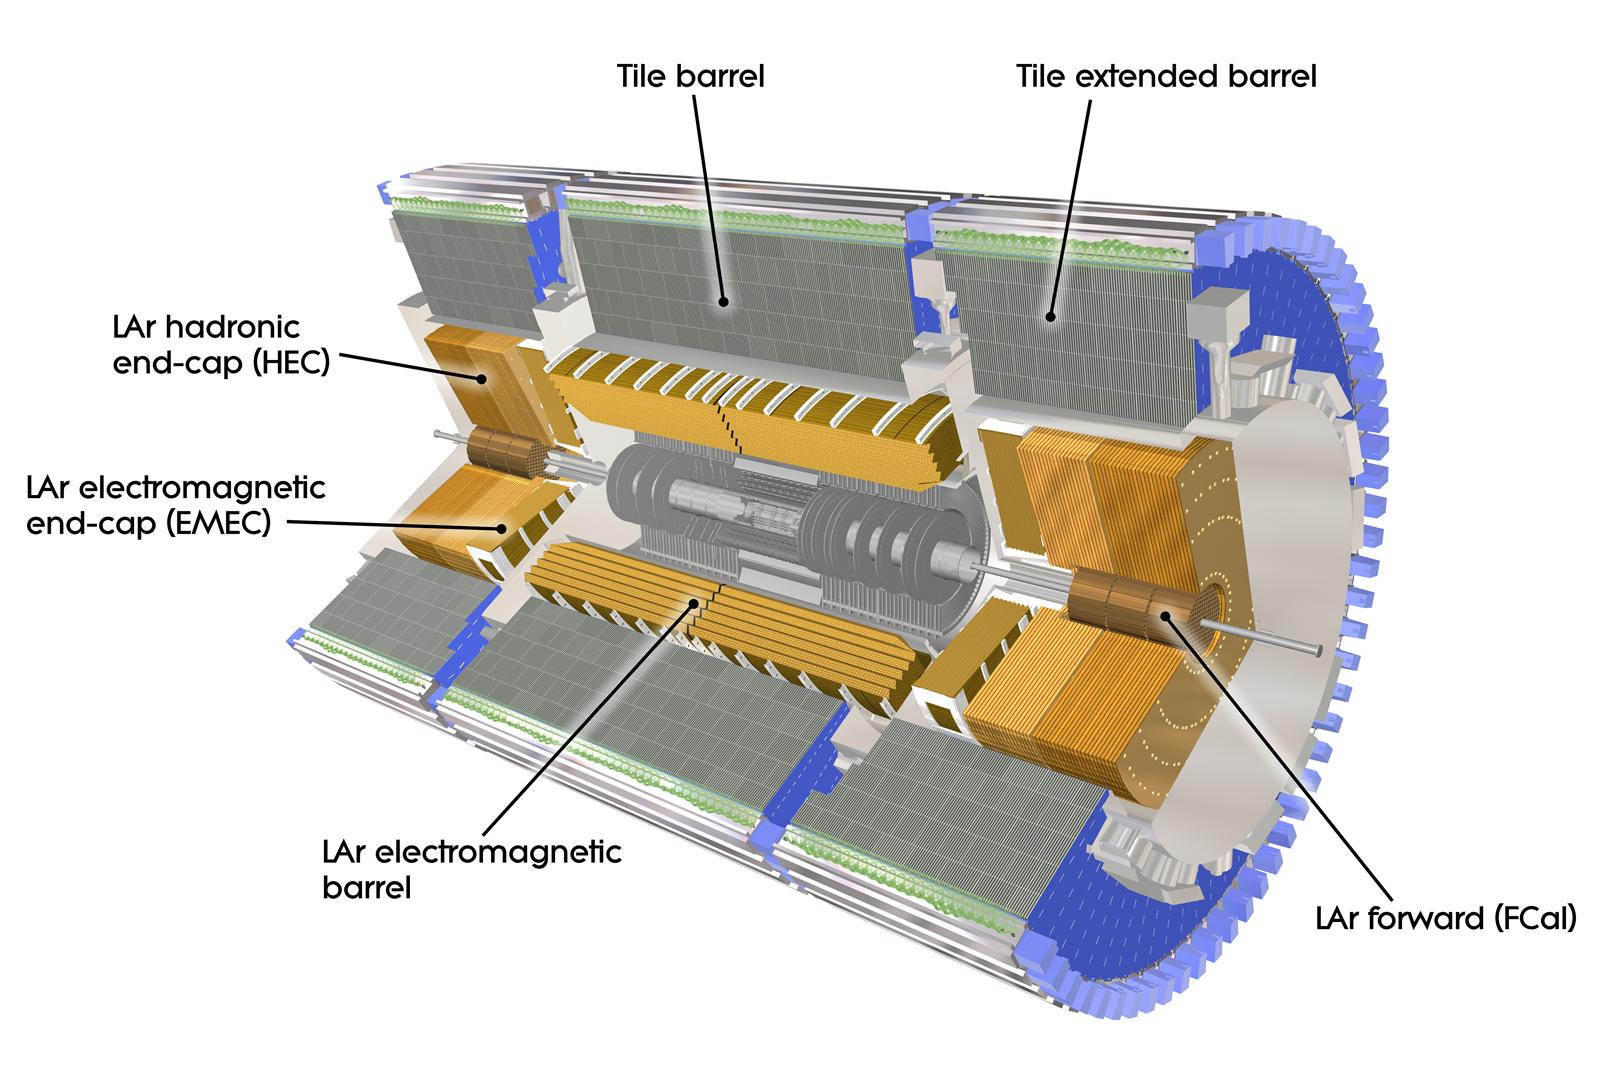
\includegraphics[width=0.7\textwidth]{calorimeters.jpg}
\label{fig:detector:calo}
\caption{A computer generated image of the ATLAS calorimeter system, showing the locations of each different subdetector. Copyright CERN.}
\end{figure}

%%%%%%%%%%%%%%%% 


\subsection{Electromagnetic Calorimeter}

Like many of the other detectors, the ECal is composed of two main sections; the barrel and the endcaps~\cite{ATLASPaper}. The barrel covers the range $|\eta| < 1.475$, and occupy the space between 2.8 m and 4 m from the beamline. The detector is a total of 6.4 m long. Both use lead as the passive layer and liquid argon as the active material. A presampler covers the entire $\eta$ range of the barrel.

The endcaps consist of two wheels, on either side of the detector, and cover the range $1.375 < |\eta| < 3.2$ and occupy the region between 330 mm and 2098 mm from the beamline\footnote{Note that this is the first detector component listed that sits outside of the tracker volume in $z$, and so is not limited by the tracker's radial size.} A presampler also covers the region in front of the endcap.

The LAr calorimeters all operate via the measurement of ionization~\cite{Detectors,Wigmans}. As particles--- particularly photons and electrons which interact predominantly electromagnetically--- interact with the liquid argon, they knock free electrons and create ions. The high voltage applied across opposite ends of the detector drifts the free electrons to one side, where they can be measured. The passive lead layers promote electromagnetic showering which can be read out by the active material, while also providing a large number of radiation lengths to absorb the energy of these particles.

The barrel system is composed of 2048 so-called ``accordion-shaped'' absorbers, instrumented with interleaved readout electrodes~\cite{ATLASPaper}. The characteristic accordion shape, displayed in Figure~\ref{fig:detector:lar-accordion}, is designed to reduce the drift time after a particle interacts but before the ionization energy has been collected. Depending on the $\eta$, there are between 3 and 4 separately read-out layers, in addition to the presampler, in each module. The size of the detector cells which are read out depends on the layer, as shown in Figure~\ref{fig:detector:lar-module}. 

%%%%%%%%%%%%%%%%

\begin{figure}
\centering
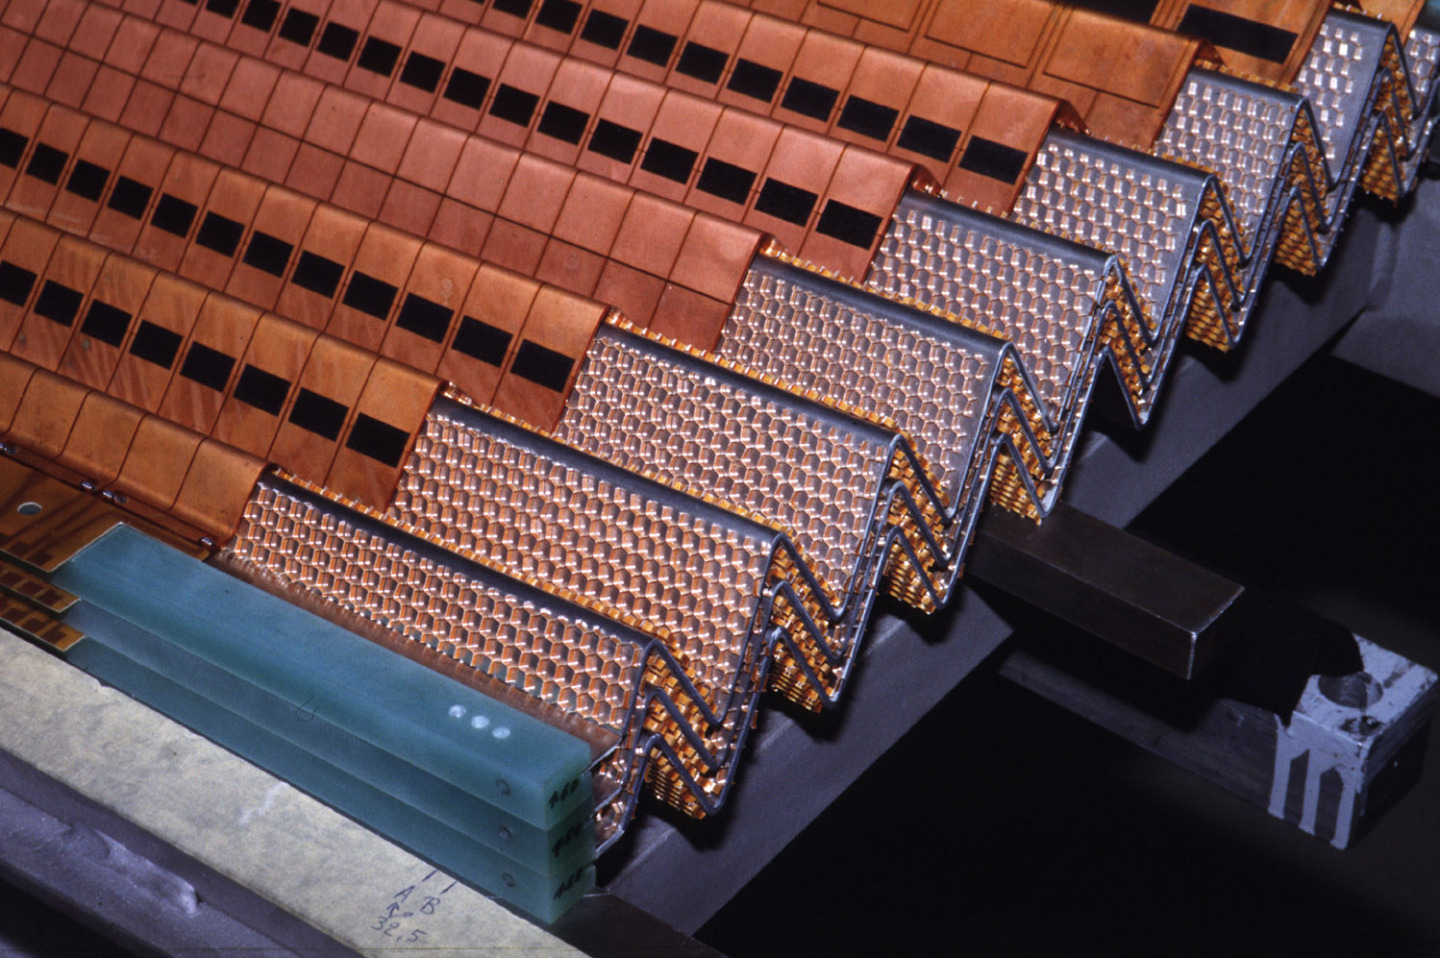
\includegraphics[width=0.7\textwidth]{lar-accordion.jpg}
\label{fig:detector:lar-accordion}
\caption{A photograph of the accordion structure used in the LAr barrel. Copyright CERN.}
\end{figure}

%%%%%%%%%%%%%%%% 

%%%%%%%%%%%%%%%%

\begin{figure}
\centering
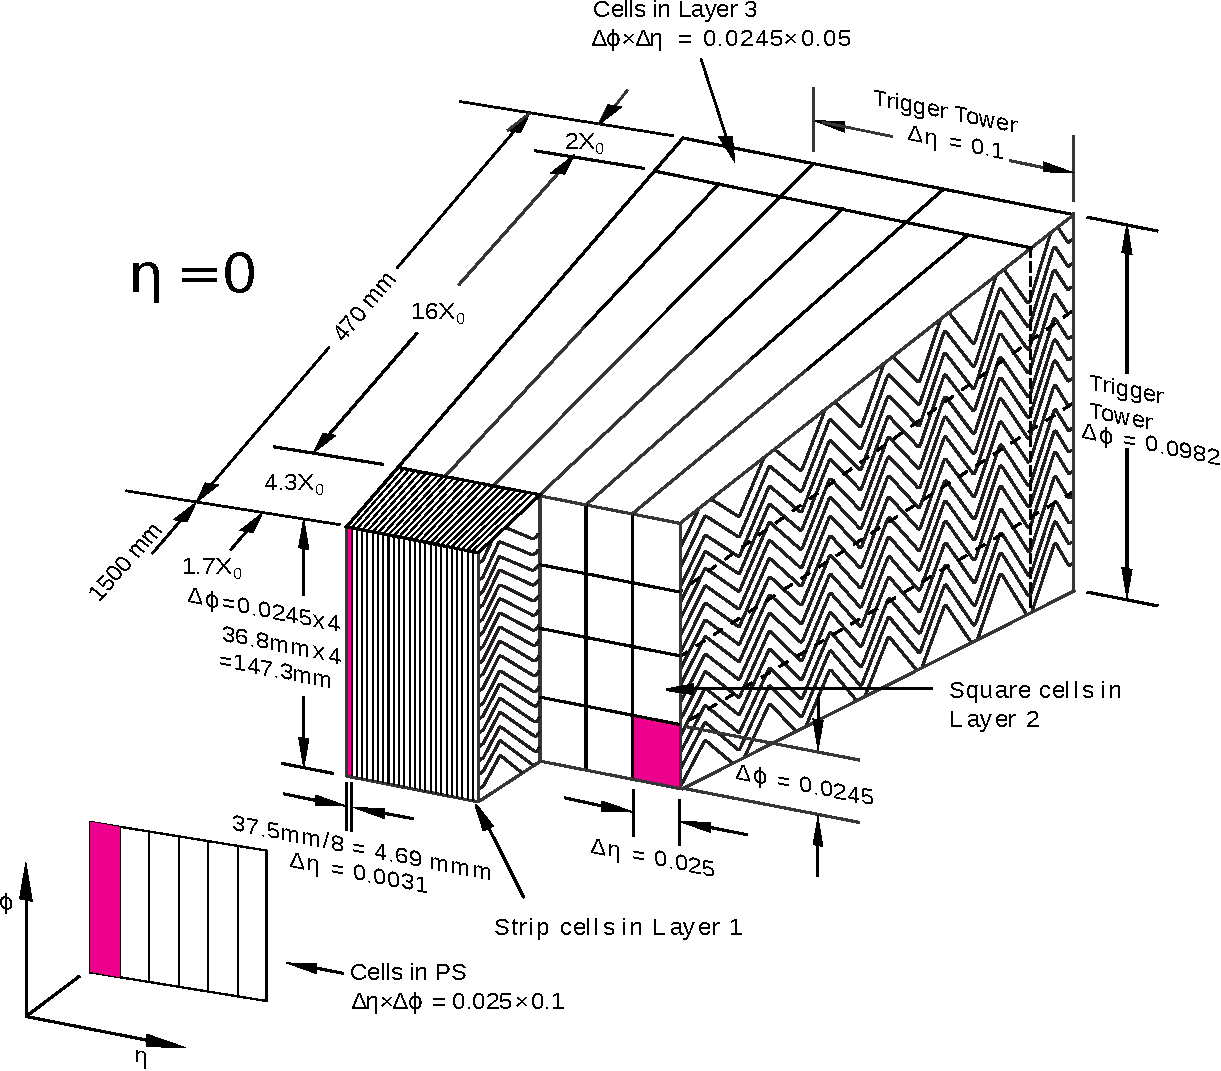
\includegraphics[width=0.7\textwidth]{lar-module.pdf}
\label{fig:detector:lar-module}
\caption{A drawing of a LAr module near $\eta = 0$. The relative size of each layer in the module, in both length and radiation lengths, is shown.}
\end{figure}

%%%%%%%%%%%%%%%% 



The endcap follows a similar design, separated into two sub-wheels per wheel~\cite{ATLASPaper}. The outer wheel (at lower values of $|\eta|$) is composed of 768 absorbers with three layers, and the inner wheel (at higher values of $|\eta|$) is composed of 256 absorbers with only two layers. The granularity of the outer wheel is similar to that of the barrel calorimeter, but the inner wheel has a coarser granularity.\footnote{Note though that while the granularity is worse in $\eta$, the coordinate is asymptotic as $\theta$ increase and the physical granularity of the inner wheel is not actually decreasing.} Figure~\ref{fig:detector:lar-endcap} shows a photograph of one of the LAr endcaps after its installation in the detector.


%%%%%%%%%%%%%%%%

\begin{figure}
\centering
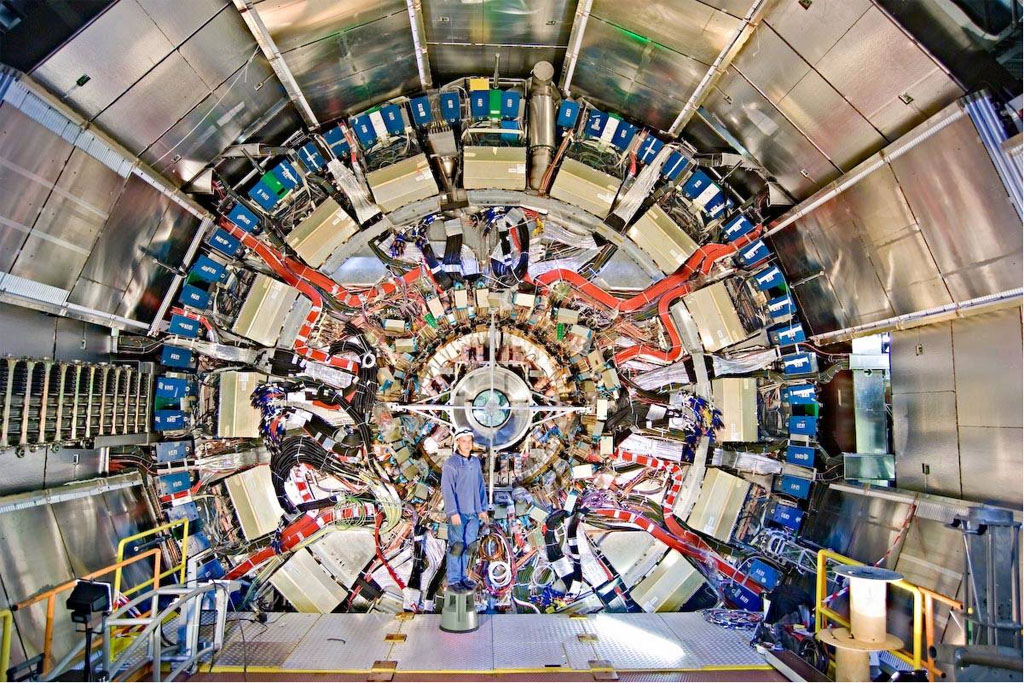
\includegraphics[width=0.7\textwidth]{lar-endcap.jpg}
\label{fig:detector:lar-endcap}
\caption{A photograph of the LAr endcap after installation in the cryostat system. Copyright CERN.}
\end{figure}

%%%%%%%%%%%%%%%% 

Both detectors operate at voltages of approximately 2 kV~\cite{ATLASPaper}. The barrel occupies a cryostat shared with the solenoid, and is cooled by a nitrogen refrigerator system which operates at 80 K. The endcaps each share a cryostat with the HEC and FCal, and are cooled by a similar nitrogen system.

A benefit of using liquid argon as a readout material is that it is readily purified and relatively inexpensive and so can easily be used in large volumes. A drawback is the long collection time of the ionization energy, typically of order 450 ns, which is complicated by the LHC's design of collisions every 25 ns~\cite{ATLASPaper,LARPaper}. This means that after a particle has left an energy deposit in the calorimeter in one bunch crossing, it remains for up to 16 subsequent bunch crossings. This effect is referred to as ``out-of-time'' pileup. One solution to this issue is to exploit the very consistent and well understood characteristics of the ionization pulse, and to shape it (via the readout electronics) to compensate for out-of-time pileup. This is demonstrated in Figure~\ref{fig:detector:lar-pulse}: a bipolar $CR -(RC)^2$ analogue filter generates a fast time constant for the rise and fall (13 ns), resulting in a negative energy portion of the pulse~\cite{LARPaper}. This negative energy portion has the same integrated area as the positive portion: on average, the negative portion should cancel the in-time component of pileup from subsequent collisions~\cite{Loch}. The very predictable pulse shape also simplifies the readout: only the first five points need to be read out to predict the full shape, as shown in Figure~\ref{fig:detector:lar-pulse-2}. Of course, the ECal is also susceptible to in-time pileup, as the detector does not have sufficient position resolution to identify whether an energy deposit occured from the primary hard-scatter or additional primary vertices.

%%%%%%%%%%%%%%%%

\begin{figure}
\centering
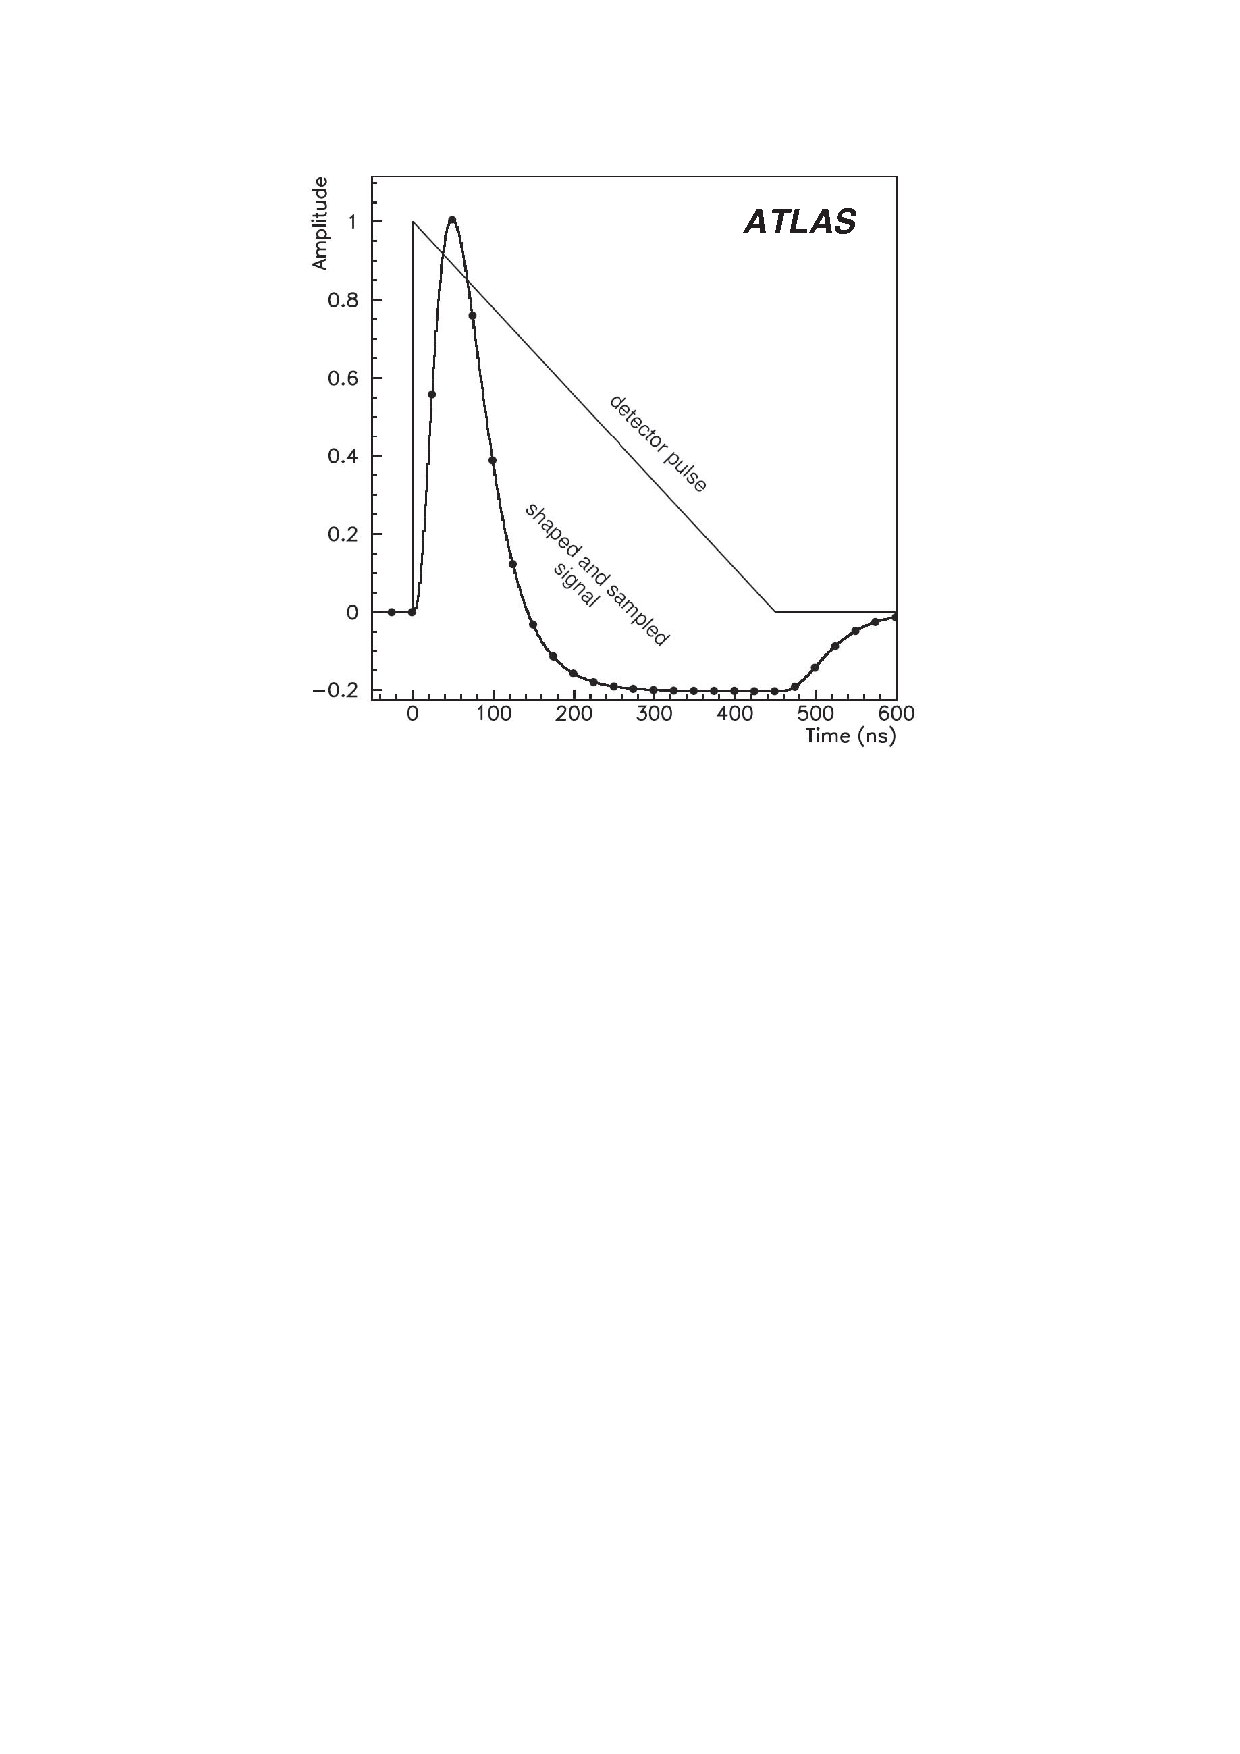
\includegraphics[width=0.7\textwidth]{lar-pulse.pdf}
\label{fig:detector:lar-pulse}
\caption{A plot of the LAr ionization pulse and the shaped output from the frontend electronics, including the negative energy region.}
\end{figure}

%%%%%%%%%%%%%%%% 

%%%%%%%%%%%%%%%%

\begin{figure}
\centering
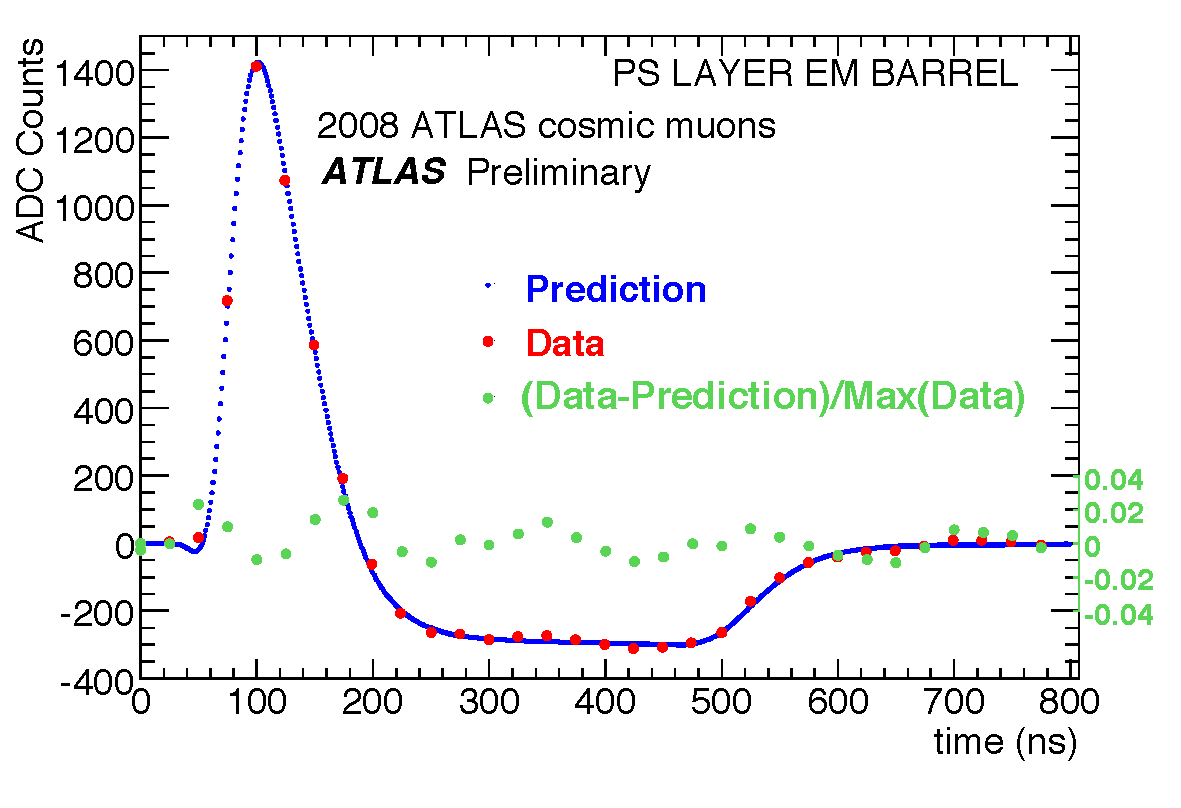
\includegraphics[width=0.7\textwidth]{lar-pulse-2.pdf}
\label{fig:detector:lar-pulse-2}
\caption{A plot the measured and predicted LAr energy distributions during a 2008 cosmic ray run.}
\end{figure}

%%%%%%%%%%%%%%%% 

As the liquid argon in the detector can be continuously filtered, there is no danger of damage due to radiation (in contrast to the CMS homogenous crystal calorimeter, which `darkens' over time and portions of which will require replacement in time). Future upgrades include the goal of reading out at a higher rate and with potentially greater granularity, especially at the trigger level.



\subsection{Hadronic Calorimeter}

The Hadronic Calorimeter is composed of four subsystems: the tile barrel, the tile extended barrel, the LAr hadronic endcap, and the LAr forward calorimeter. 

The tile systems extend to $|\eta| < 1.7$ and sit behind the LAr electromagnetic calorimeter~\cite{ATLASPaper,Tile}. The barrel detector is 5.8 m long, and each of the extended barrels are 2.6m long. The detectors each have an inner radius of 2.28 m and an outer radius of 4.25 m. The combined detector is shown, after installation the ATLAS cavern, in Figure~\ref{fig:detector:barrel-tile}. The detectors are composed of 64 wedge-shaped modules with size $\Delta\phi \approx 0.1$, an example of which is pictured in Figure~\ref{fig:detector:tile-wedge}. The detector is composed of alternating layers of steel plates and plastic scintillating tiles: by volume the steel-to-tile ratio is approximately 4.7:1 and is almost exactly periodic. The detector operates via similar principles to that of the ECal: particles (which at this depth in the detector are mostly hadrons) interact with the steel and produce showers of lower energy particles. These particles proceed through the scintillator: as they pass through a material where the speed of light is lower than their current speed, they emit scintillation light, which can be collected by readout fibers and read out by photomultiplier tubes~\cite{Wigmans,Detectors,Tile}. \editnote{CHECK ME I THINK THIS IS WRONG} An example of one of the scintillating tiles is pictured in Figure~\ref{fig:detector:actualtile}. Like the ECal, the tile calorimeter contains three independently readout layers, which provies information about the longitudinal development of the particle shower. The detectectors are readout in $\Delta \eta \times \Delta\phi$ cells of approximately  $0.1 \times 0.1$ for the front two layers  and $0.2 \times 0.1$ for the third layer.

Unlike the LAr systems, the tile calorimeters have a fairly quick readout and are not affected by out-of-time pileup. Because the tile system sits behind so many other detectors, and pileup particles are generally rather low-energy to begin with and therefore usually stopped by the upstream detectors, even in-time pileup is expected to have a much lower effect than on the ECal.

The hadronic endcap system is similar to the ECal, but is composed of alternating layers of copper and liquid-argon with a flat design (in contrast to the ECal's accordion shape)~\cite{ATLASPaper}. The detectors occupy the range $1.5 < |\eta| < 3.2$, and they share the end-cap cryostats with the EMEC and FCal.  Each HEC endcap is composed of two wheels, each of of which has two longitudinal layers. Each of the four wheels is cylindrical, with an outer radius of 2.03 m, and each of the wheels is composed of 32 wedge-shaped modules. The read-out cells have size $\Delta \eta \times \Delta\phi = 0.1 \times 0.1$ for $|\eta| < 2.5$, and $0.2 \times 0.2$ for larger values. The LAr ionization readout uses high-voltage set to 1800 V.

The ATLAS forward calorimeters are the final devices in the end-cap cryostats, and sit in the highest pseudorapidity, covering $3.1 < |\eta| < 4.9$~\cite{ATLASPaper}. The FCal is composed of three 45 cm modules: FCal1 is an electromagnetic module, and FCal2 and FCal3 are hadronic modules. Copper is used as the absorber in FCal1, and tungsten is used in FCal2/3. All three use liquid argon as the active medium.

The HCal systems are all expected to perform very well in future LHC runs, even with increased pileup conditions. Upgrades to some of the readout systems to enable more rapid and more regular collection of data are the main goals in preparation for higher luminosity operations.

%%%%%%%%%%%%%%%%

\begin{figure}
\centering
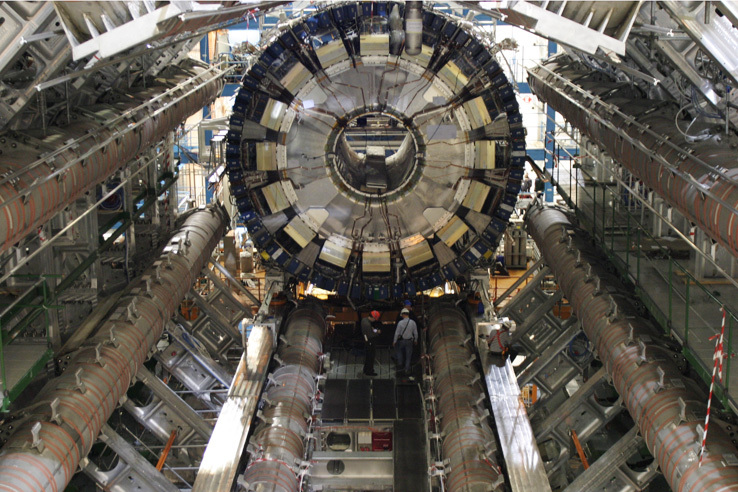
\includegraphics[width=0.7\textwidth]{tile.jpg}
\label{fig:detector:barrel-tile}
\caption{A photograph of the installation of the barrel tile calorimeter. Copyright CERN.}
\end{figure}

%%%%%%%%%%%%%%%% 

%%%%%%%%%%%%%%%%

\begin{figure}
\centering
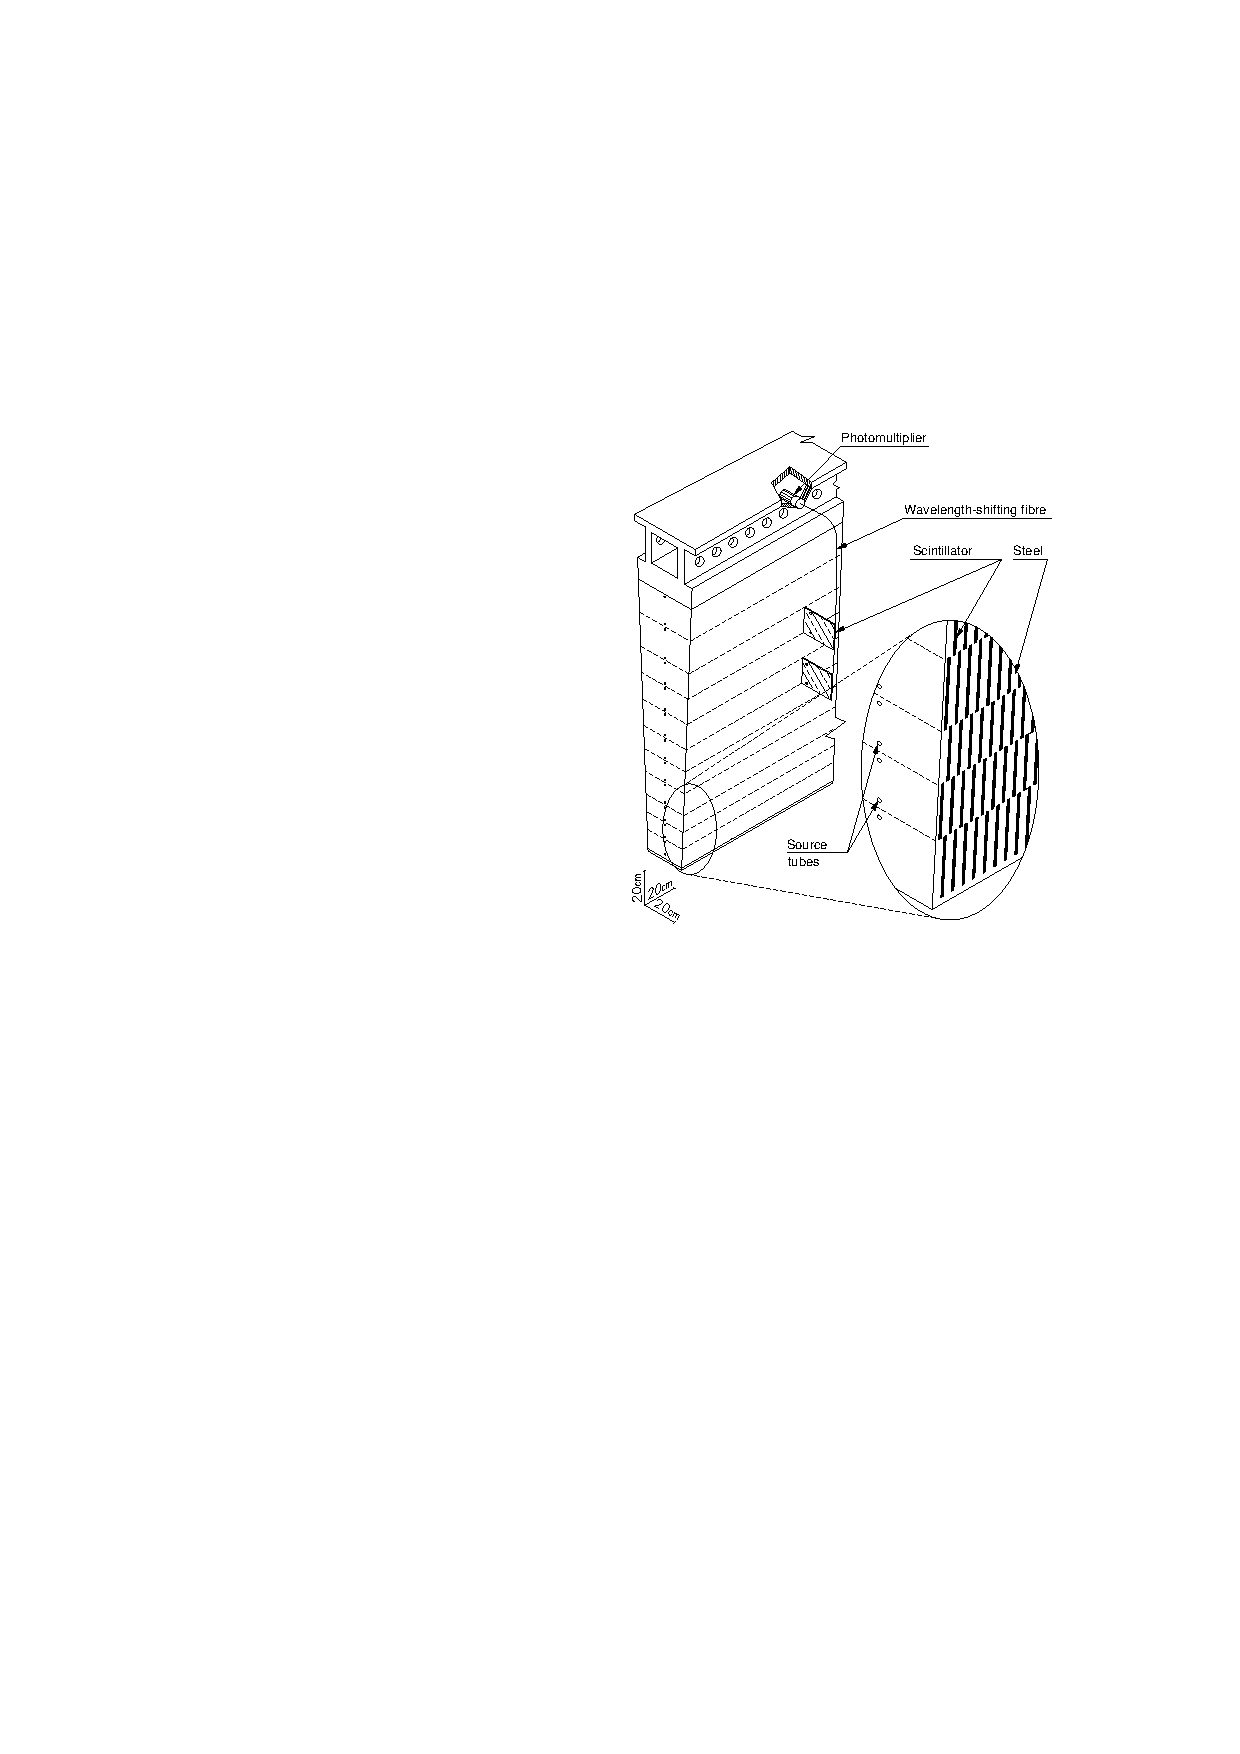
\includegraphics[width=0.7\textwidth]{tile-wedge.pdf}
\label{fig:detector:tile-wedge}
\caption{A drawing of one wedge of the tile detector.}
\end{figure}

%%%%%%%%%%%%%%%% 

%%%%%%%%%%%%%%%%

\begin{figure}
\centering
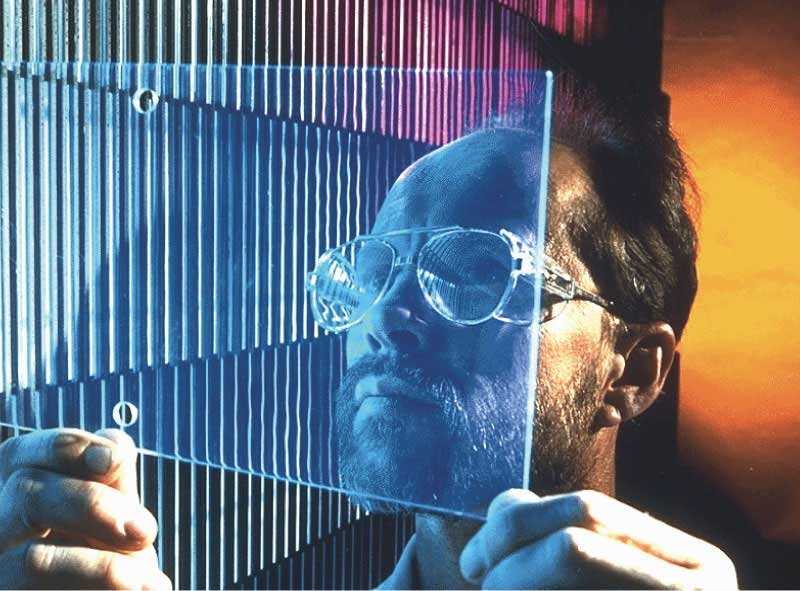
\includegraphics[width=0.7\textwidth]{tile-actualtile.jpg}
\label{fig:detector:actualtile}
\caption{A photograph of one of the scintillating tiles which give the tile calorimeter its name. Copyright CERN.}
\end{figure}

%%%%%%%%%%%%%%%% 




\section{Muon Spectrometer}

The Muon Spectrometer (MS) is the outermost detector in ATLAS~\cite{ATLASPaper}. It is designed to accurately reconstruct charged particles which exit the calorimeters out to $|\eta| < 2.7$, and can trigger on these particles to $|\eta| < 2.4$. A break for calorimeter and cryostat servies at $\eta \approx 0$ reduces the efficiency for vertical muon reconstruction.  Unlike the other detectors, which are designed to measure many different types of particles, in practice the goal of the muon spectrometer, as its name suggests, is to measure only muons, as those are typically the only particles which interact so weakly that they can pass through the calorimeter systems. The MS is capable of reconstructing tracks independently, but muon reconstruction is typically performed in a ``combined'' mode of operation, where independently reconstructed ID and MS tracks are matched to create muon candidates with improved momentum measurements. Because the toroid magnets bend particles in a direction perpendicular to that of the solenoid surrounding the ID, the measurements of the ID and MS are largely independent and increase the precision of the measurement. This is contrast to the CMS muon system, which only provides a ``tag'' which labels the muon and the ID performs the full momentum measurement.

The different subsystems of the MS are shown in Figures~\ref{fig:detector:ms} and \ref{fig:detector:ms-eta} as a computer-generated image of the whole detector and as a schematic drawing in the $z-\eta$ plane respectively. Note that Figure~\ref{fig:detector:ms-eta} shows the MS in the bending plane of the toroids: curved trajectories in this direction are measured to extract the momenta of particles. 


%%%%%%%%%%%%%%%%

\begin{figure}
\centering
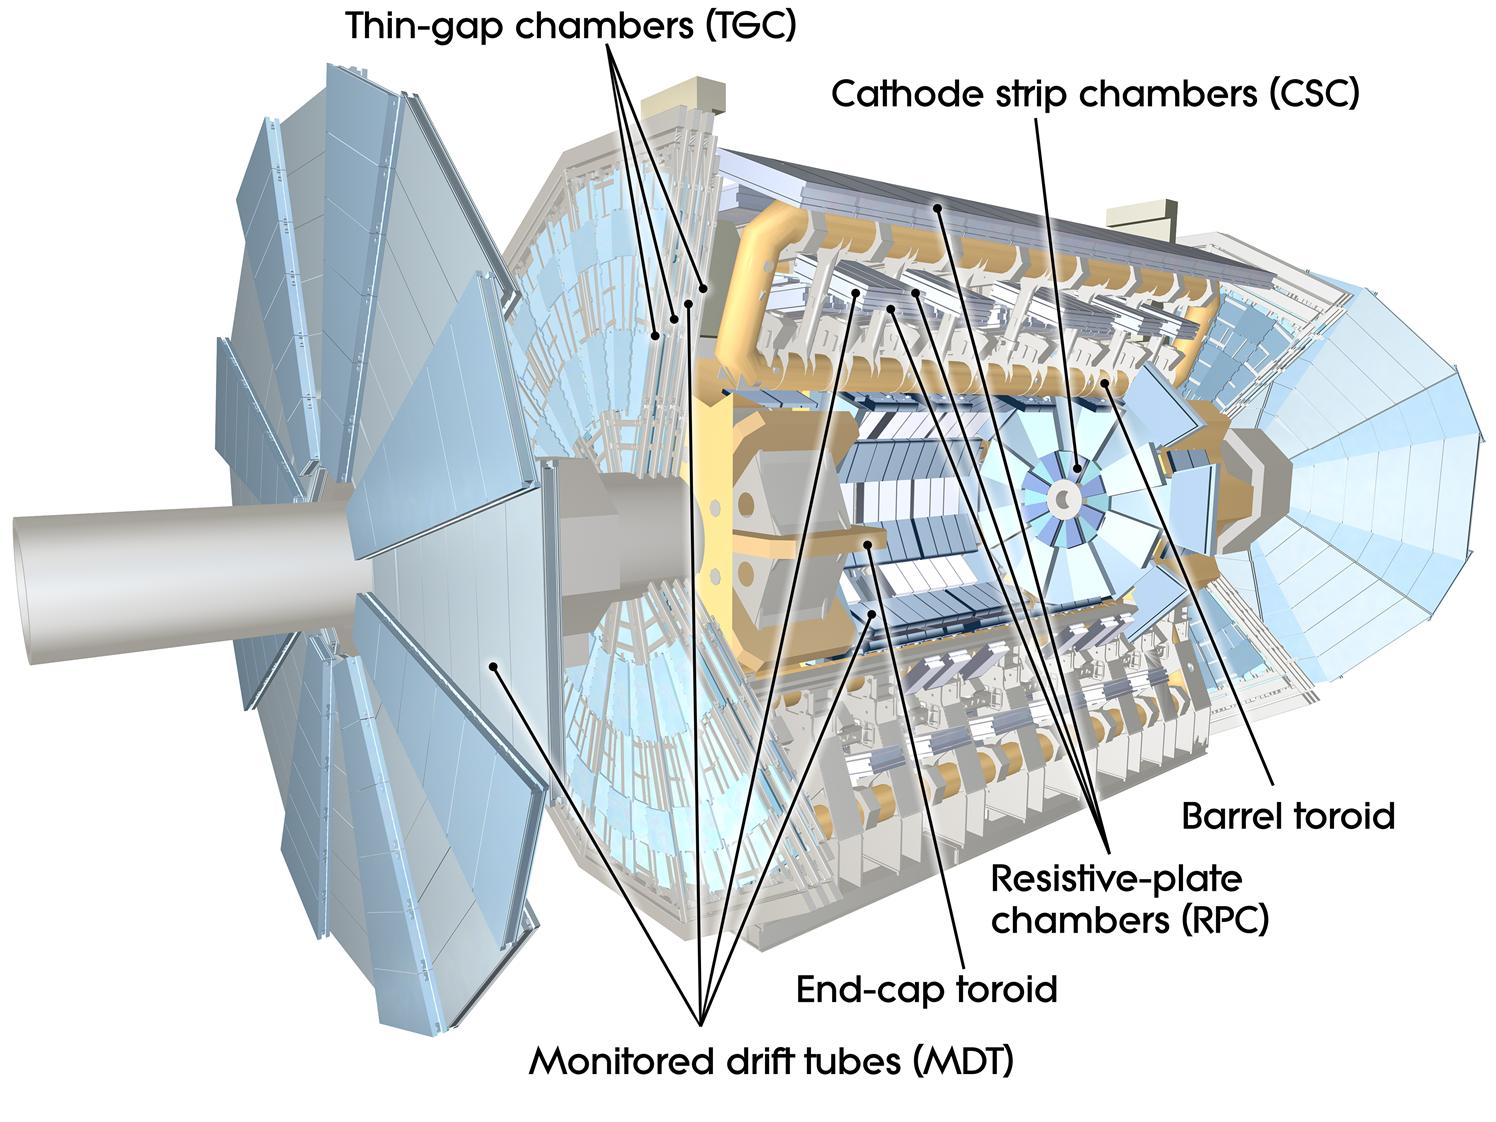
\includegraphics[width=0.7\textwidth]{muons.jpg}
\label{fig:detector:ms}
\caption{A computer generated image showing the locations of each of the muon spectrometer subsystems. Copyright CERN.}
\end{figure}

%%%%%%%%%%%%%%%% 

%%%%%%%%%%%%%%%%

\begin{figure}
\centering
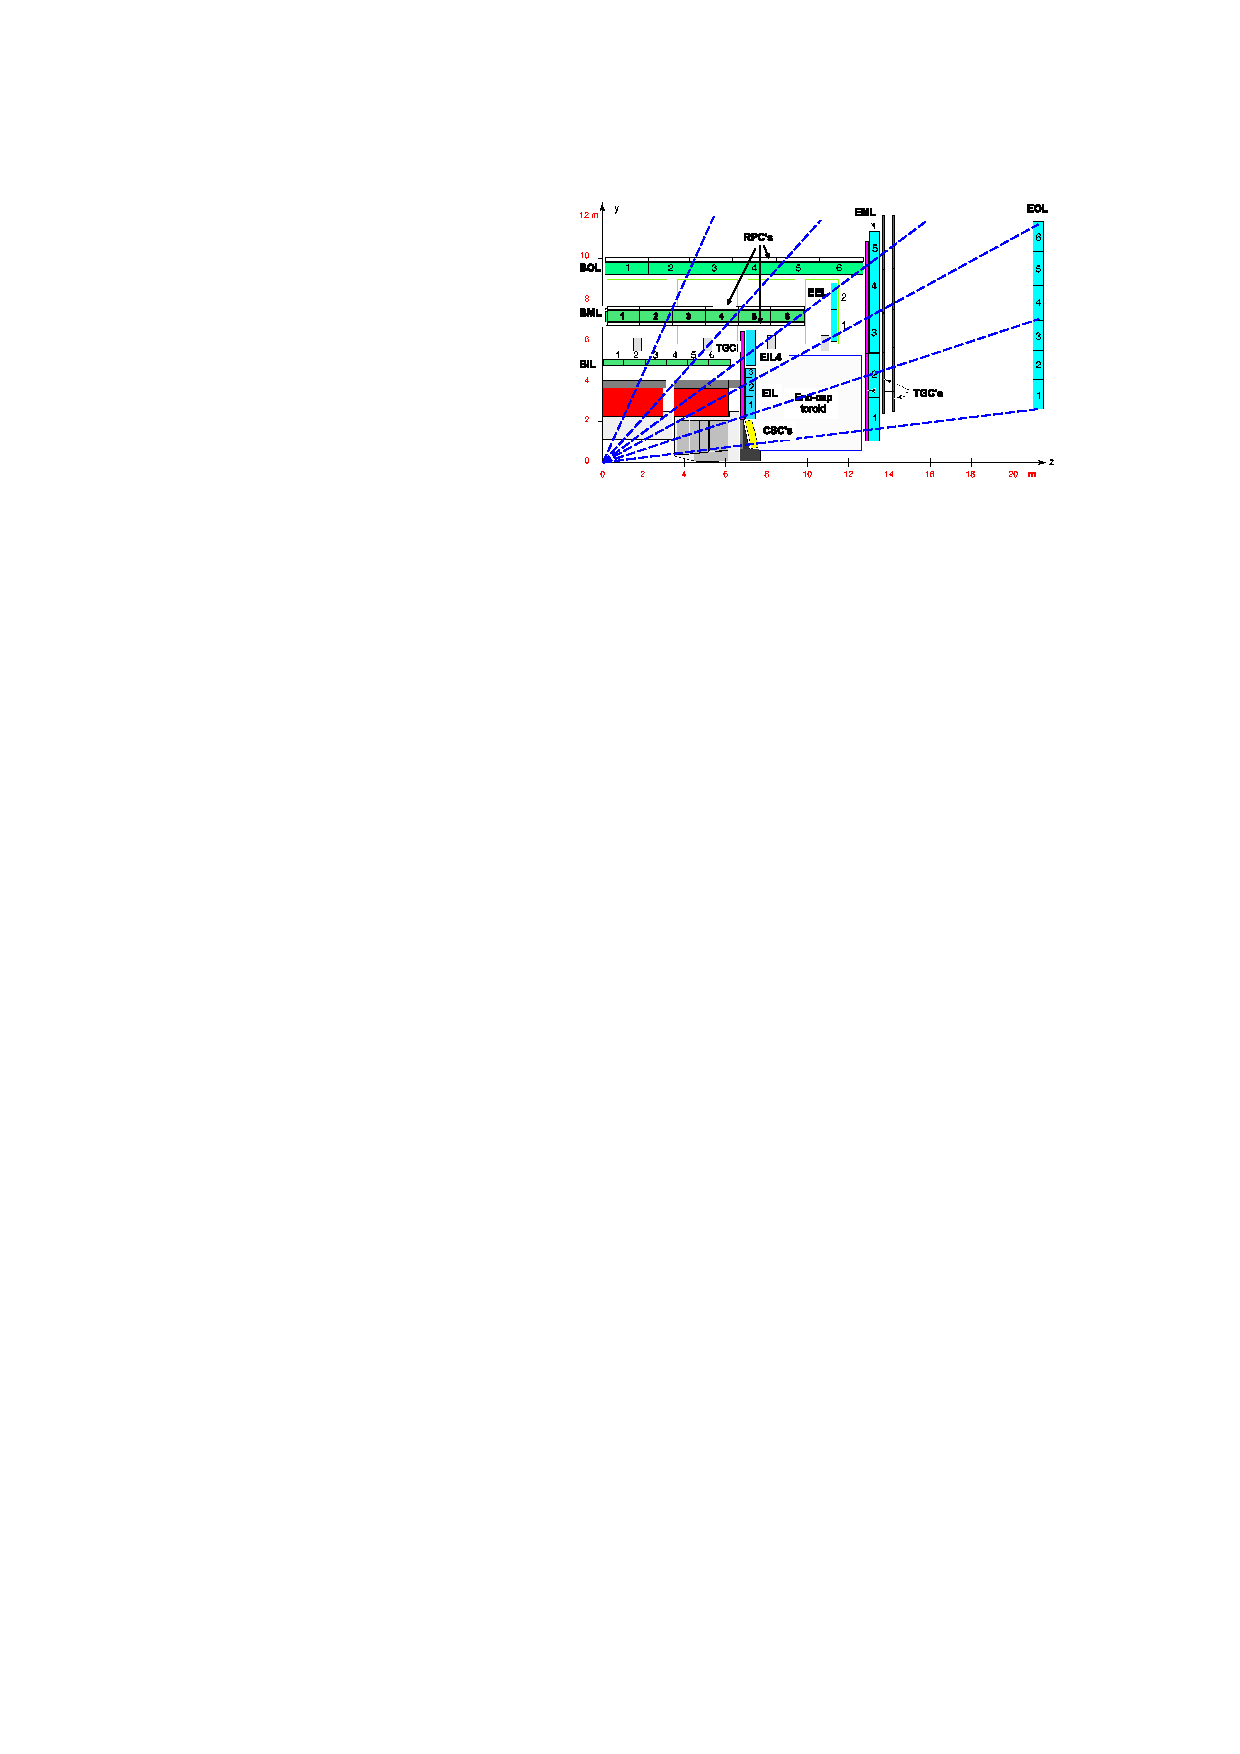
\includegraphics[width=0.7\textwidth]{muon-eta.pdf}
\label{fig:detector:ms-eta}
\caption{A drawing in the $z/\eta$ plane showing the location of the various detector subsystems in the MS. This is the bending plane of the toroids, so infinite momentum particles would have straight trajectories in this view and others would be curved.}
\end{figure}

%%%%%%%%%%%%%%%% 

The largest subsystem of the MS are the Monitored Drift Tube chambers (MDT's), which provide precision measurements of charged particle hits~\cite{ATLASPaper}. There are 1088 MDT chambers in the detector, covering a total area of 5500 m$^2$. Chambers are composed of several layers of the eponymous tubes, and the precise number of tubes in each chamber varies between 48 and 432. The chambers are arranged into three layers in the barrel and three wheels in the endcap (though at high $\eta$ values only two layers of MDT are used due to the higher particle flux). The tubes themselves are proportional drift chambers with an Ar/CO$_2$ gas mixture at $93\%/7\%$ respectively~\cite{ATLASPaper,Detectors}. Ionization electrons are collected by a central tungsten-rhenium wire, held at a potential of 3080 V. Similar to the TRT described in Section~\ref{detector:ID:TRT}, the drift tubes provide only one coordinate measurement, this time in the $z$ direction to take advantage of the toroid bending axis. The non-measured coordinate of a hit is provided by the triggering detectors, described below. The MDTs provide a typical resolution of 35 $\mu$m in the $z$ direction, and muons typically cross 20 tubes as they are measured. The maximum readout time of an MDT is approximately 700 ns-- to prevent overlapping measurements from different collisions, the readout system implements a dead-time after the first detection of charge.
 
Cathode-Strip Chambers (CSC's) sit in the forward region of $2.0 < |\eta| < 2.7$, and are used in track reconstruction in the $2.0 < |\eta| < 2.7$ region where the MDTs have only two layers, both of which appear after the CSC~\cite{ATLASPaper}. The CSC chambers are arranged in four consecutive planes in each wheel, for a total of 32 chambers; each plane is composed of perpendicular strips which allow for the measurement of both coordinates of a hit. The CSCs provide fewer hits than an equivalent layer of MDTs, but have fewer readout inefficiencies due to their faster response time. The CSC's are multiwire proportional chambers whose wires are oriented in the radial direction. The anodes of the detector are the wires, and the sides (in the $R$ and $\phi$ directions) are instrumented cathodes which readout the ionization of the Ar/CO$_2$ gas mixture (operated at $80\%/20\%$)~\cite{Detectors,ATLASPaper}. The detectors are operated at 1900 V, and have typical drift times of much less than 40 ns. The fine segmentation of the cathodes in both coordinates allows for very accurate position measurements, allowing for typical resolutions of 40 $\mu$m in $R$ and 5 mm in $\phi$.

In addition to the precision measurement systems, the MS contains two systems used primarily for triggering. The Resistive Plate Chambers (RPC) are used in the barrel region of $|\eta| < 1.05$, and Thin Gap Chambers (TGC) are used in the endcap ($1.05 < |\eta| < 2.4$). The detectors are meant to measure the non-bending coordinate of the track to complement the MDT measurements, and to provide a complete, fast, and coarse tracking for use in the trigger. 

RPCs are parallel plate ionization detectors, and measure hits through the ionization of gas~\cite{Detectors,ATLASPaper}. The plates are kept 2 mm from each other, with an electric field of 4.9k kV/mm. The plates are segmented for the purposes of readout, allowing for local determination of hit coordinates. RPCs are typically paired with MDT stations, allowing the non-bending coordinate measured by the RPC to be used by the MDT hit. The RPCs have a typical hit resolution of 10 mm in $z$ and $\phi$, and muons typically cross 6 detectors. 

TGCs are multi-wire proportional chambers similar in some respects to the CSCs. The bending coordinate is measured by collection of charge on the TGC wire, while the other is measured by radial strips in the cathode. The detector is arranged into circular disks mounted in two concentric rings. The TGCs have a typical hit resolution of $2-6$ mm in $R$ and 3-7 mm in $\phi$, and muons typically cross 9 detectors.

While the vast majority of the use of the MS comes from its measurement of muons, it provides some additional use in the study of hadronic physics (besides measuring muons from semi-leptonic decays) by enabling the measurement of punch-through~\cite{JES2010}. Some jets--- either because of parton shower fluctuations or because they are extremely high energy--- are not contained entirely by the calorimeter system. Because all the calorimeters are sampling, this means that some portion of the energy of the jet is also not measured. However, these particles can still proceed through the MS and leave hits in the detectors, as seen in Figure~\ref{fig:detector:punchthrough}. These hits can be used to create on-average corrections for punchthrough, and can thereby improve the energy measurement of jets in an unusual way.

While the detectors of the MS are not expected to need replacement due to radiation (the choice of detector gas was often motivated to guarantee this robustness), issues of readout optimization and occupancy do arise at higher luminosity. In particular, the CSC readout has been completely redesigned for Run II in order to provide measurements at a much higher rate in order to assist in muon triggering. \editnote{Is this correct?}

%%%%%%%%%%%%%%%%

\begin{figure}
\centering
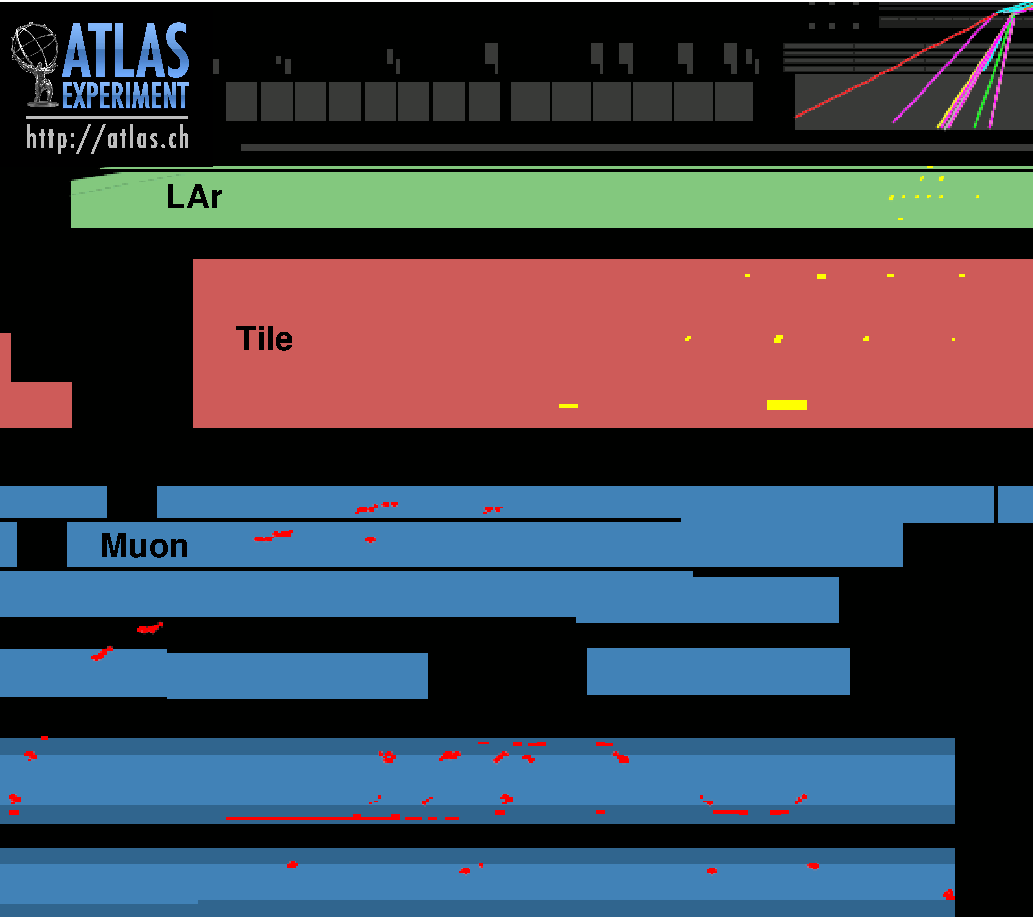
\includegraphics[width=0.7\textwidth]{punchthrough.pdf}
\label{fig:detector:punchthrough}
\caption{A portion of an event display showing a high $p_T$ jet (176 GeV) with 128 measured hits in the muon spectrometer.}
\end{figure}

%%%%%%%%%%%%%%%% 

\section{Forward Detectors}

In addition to the main detectors described in the previous sections, several forward detectors (some even located outside of the main volume) provide additional information used in luminosity measurements and some triggering applications~\cite{ATLASPaper}. The luminosity measurements are particularly critical for searches for new physics, and for understanding of the accelerator conditions. The radiation-hard diamond Beam Conditions Monitor (BCM), for example, is place at $\pm$ 1.84 m in $z$ and use a fast response time (2 ns) to distinguish between collision events and beam anomalies. The Minimum-Bias Trigger Scintillators (MBTS), placed at $\pm 3.56$m, are fast-responding plastic scintillators used to trigger on collisions that do not leave large energy signatures in the central detectors. The LUminosity measurement using a Cerenkov Integrating Detector (LUCID) follows the terrible naming conventions developed by ASCOT and ATLAS. It measures the luminosity by measuring the $pp$ elastic cross-section with two very far forward detectors, placed at $\pm$ 17 m and 100 mm in $r$. The detectors consist of aluminum tubes filled with scintillating gas readout by photomultiplier tubes, enabling measurements of the luminosity to 25$\%$ precision.

\section{Triggering}

With collisions occuring every 25 ns at design luminosity, and even every 50 ns in 2012 operations, ATLAS has no chance of recording every collision. Instead, a triggering system is used to quickly identify interesting events and to mark them for later analysis\cite{ATLASPaper,Trigger2010}. This system is divided into three stages: Level 1 (L1), Level 2 (L2), and the Event Filter (EF). Each stage is designed to make a decision using some limited amount of information from the detector at a maximum rate before handing off to the next stage, which can use more information to make a better informed decision. In this manner, the initial collision rate of 40 MHz (20 MHz in 2012) is reduced to 75 kHz after the L1, 3.5 kHz at L2, and 200 Hz at EF. The listed rates were design goals for the initial running of ATLAS: in practice, as much as 400-600 Hz were accepted at EF during Run 1.

\subsection{Level 1}

The L1 trigger is unique amongst the trigger subsystems in that it is implemented entirely in custom hardware, configurable with programmable firmware~\cite{ATLASPaper,Trigger2010}. The L1 accepts information from the calorimeter and muon spectrometer systems only, as the ID information takes significantly longer to readout and is not available at the rate requried for L1 decisions.  The L1 muon triggers typically require 3 hits in coincidence in either the RPC or TGC detectors, with various $p_T$ threshholds. The calorimeter trigger system is significantly more complicated. As the high level of granularity of the detector would present rate challenges for the trigger, the calorimeter is readout in $0.1\times0.1$ towers in $\eta \times \phi$ (with worse granularity at high $\eta$), and typically ignore longitudinal segmentation. These trigger towers are used as the basis for triggers for electrons, photons, taus, jets, total transverse energy $\sum E_T$, and missing energy $\MET$. The various signatures combine the towers in different ways to create the relevant physics objects: jets, for example, are searched for with a sliding window algorithm which looks at $8\times 8$ tower regions and identifies areas with significant $E_T$. Photons and electrons typically use smaller regions, and require isolation of the signal to reduce contamination from jet backgrounds~\cite{Trigger2010}.

Information from the L1 decisions are passed to the Central Trigger Processor (CTP), and data from the detector is offloaded to on-detector buffers in case an accept signal is sent~\cite{ATLASPaper}. The CTP can store up to 256 signatures, which are various combinations of muon and calorimeter information. Once the CTP sends a decision, detector buffers are transfered to the Read-Out System (ROS) via the Read-Out Links (ROLs), each of which has a Read-Out Buffer (ROB). The areas of the detector which caused the L1 trigger to fire are passed to the L2 trigger as a Region Of Interest (ROI).

\subsection{Level 2}

The L2 and EF are collectively referred to as the High Level Trigger (HLT), as they are both written in software and run on commodity computers~\cite{ATLASPaper}. Significantly more information is available at L2 as the rate has already been reduced signficantly. L2 triggers usually operate via requesting ROIs from the L1 trigger, which indicate which regions of the detector should be further inspected. The data from these regions is read into L2, and used to construct jets, tracks, photons, and so on, which can be used to make trigger decisions. As L2 has significantly more information available than L1, the algorithms used to reconstruct these objects are much closer to the offline reconstruction.

\subsection{Event Filter}

If the L2 accepts an event, the full event is read out into the Sub-Farm Inputs (SFI) and is reconstructed with no ROI restrictions~\cite{ATLASPaper}. The Event Filter then applies algorithms designed to be very close to the offline reconstruction (for example, performing topoclustering, described in Section~\ref{jet-reconstruction:jet-inputs:topoclustering}, on the calorimeter cells to create inputs for jet clustering). The EF decision is performed for many events in parallel by a large network of computers--- typically each event takes 4 s to process, but the large size of the network allows for many events to be processed in parallel. This final refinement of the detector information allows for a further significant reduction in the rate. Each readout event is approximately 1.6 MB, and is sent by the Sub-Farm Outputs (SFO) to the CERN Tier 0 datacenter for permanent storage.


\section{Data Quality}
\label{atlas:data-quality}

The Run 1 detector conditoins enabled a very high efficiency of data collection by ATLAS. Figure~\ref{fig:detector:lumi} shows the delivered LHC luminosity in the 2011-2012 period in green, and the recorded ATLAS data in yellow, with the final usable data in blue. The overall efficiency is close to 90$\%$, indicating high uptime of all subsystems.

%%%%%%%%%%%%%%%%

\begin{figure}
\centering
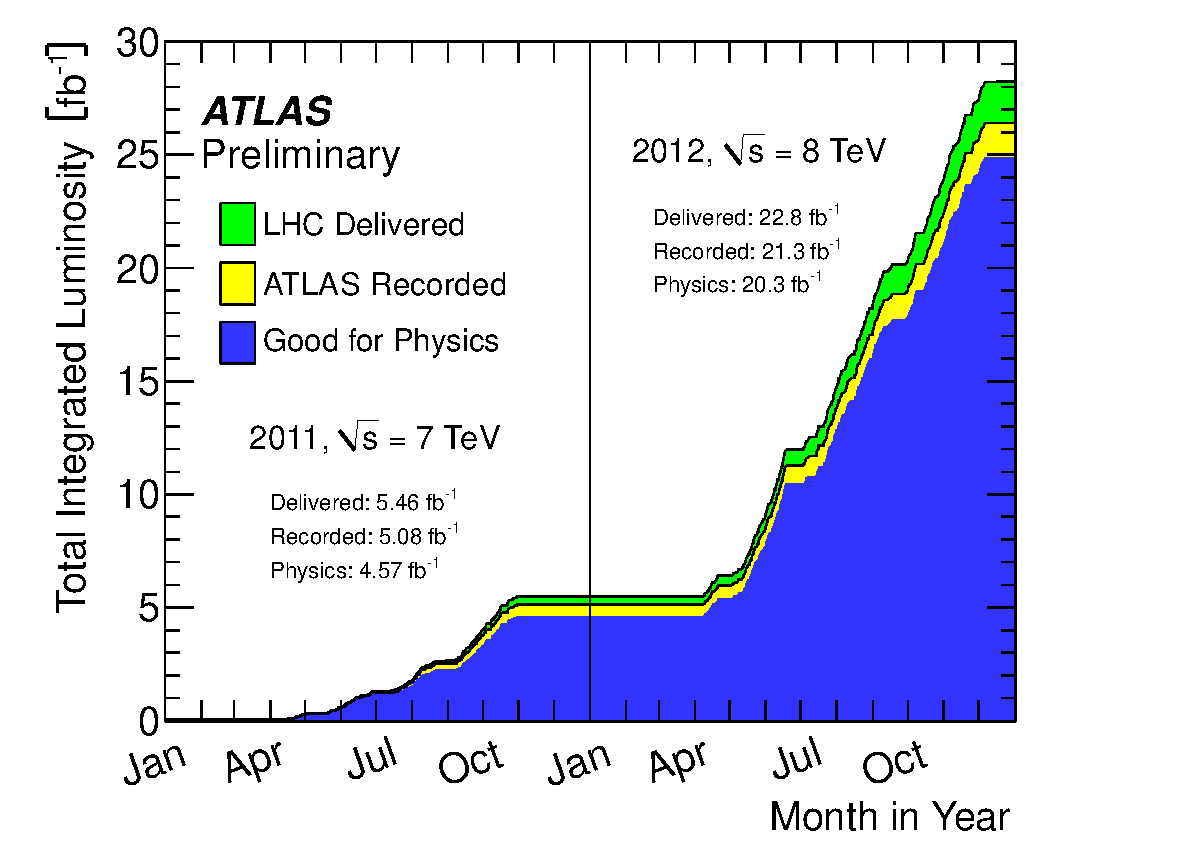
\includegraphics[width=0.7\textwidth]{atlas-lumi.pdf}
\label{fig:detector:lumi}
\caption{ATLAS recorded luminosity as a function of date in 2011 and 2012. The yellow show all data delivered by the LHC, green was recorded by ATLAS, and blue was high-quality data.}
\end{figure}

%%%%%%%%%%%%%%%% 

The detector uptime, and combined recording efficiency, is displayed in Figure~\ref{fig:detector:uptime}. All detector subsystems reported a very high uptime, with many detectors recovering data previously marked as `bad' by correcting flagged data in offline reconstruction. The remaining large portion of the inefficiency comes from the so-called ``warm start'' period, where the ATLAS pixel detector (and in early parts of the run also the SCT) ramps up its HV power supplies and preamplifiers only after the LHC has declared stable beams.

The LAr and Tile detectors critical to the hadronic analyses in this thesis both suffered several types of errors during operations. Most LAr errors were due to high-voltage power supply trips which disabled modules while the power supplies automatically recovered; most tile issues were related to problems with the low-voltage power supplies. Both of these errors were flagged during data taking so that affected events could be properly vetoed (in the case of the LAr issues) or corrected (in the case of the Tile).

%%%%%%%%%%%%%%%%

\begin{figure}
\centering
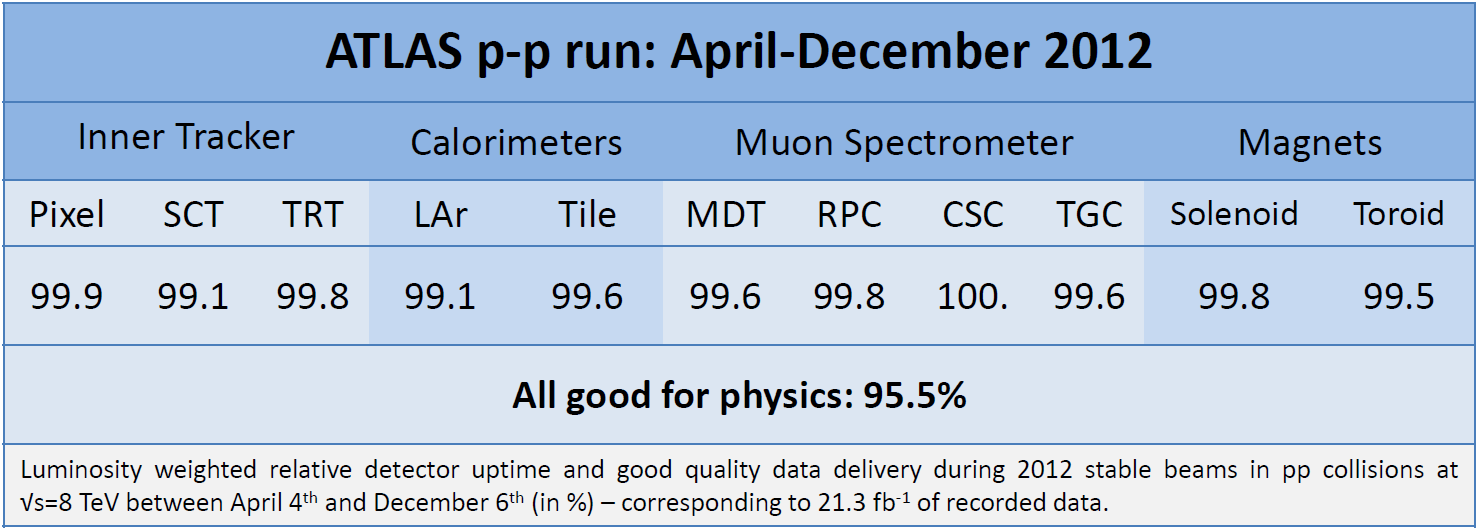
\includegraphics[width=0.7\textwidth]{DQ-eff-table2012pp-AprilDecember2012}
\label{fig:detector:uptime}
\caption{ATLAS subdetector uptime during 2012 data taking.}
\end{figure}

%%%%%%%%%%%%%%%% 
